% !TeX encoding = UTF-8
% !TeX spellcheck = en_US
% !BIB program=biber
\PassOptionsToPackage{dvipsnames}{xcolor}
\documentclass[journal]{IEEEtran}




\usepackage{etoolbox}

\usepackage{xr}
\externaldocument{supplementary}

\usepackage[%
style=numeric-comp,%
sortcites=true,%
sorting=none,%
url=false,%
doi=false,%
eprint=false,%
isbn=false,%
]{biblatex}
\addbibresource{abrv.bib}
\addbibresource{paper.bib}


\usepackage{graphicx}
\graphicspath{{./img/}}
\usepackage[labelformat=simple]{subcaption}
\captionsetup{font=footnotesize, labelfont={bf}, labelsep=period}
\renewcommand\thesubfigure{(\alph{subfigure})}
\renewcommand\thesubtable{(\alph{subtable})}

\newcommand{\boximg}[2]{\parbox[c]{#1\subfigsz}{\includegraphics[width=#1\subfigsz]{#2}}}

\usepackage{tikz}
\usepackage{pgfplots}
\usepackage{pgfplotstable}
\pgfplotsset{compat=1.16,
  grid style=dashed,
  ymajorgrids=true,
}

\newlength{\subfigsz}

\usetikzlibrary{
  calc,
  shapes,
  arrows,
  shadows,
  positioning,
  decorations.shapes,
  decorations.markings,
  fit,
  bayesnet,
  matrix,
}

\usepgfplotslibrary{
  groupplots,
  colorbrewer,
  statistics,
  fillbetween,
}


\usepackage{booktabs}           %
\usepackage{multirow}
\usepackage{arydshln}           %


\usepackage{siunitx}
\sisetup{
  separate-uncertainty,
  table-format=1.2(3),
  detect-all,
}
\robustify\bf

\makeatletter
\def\adl@drawiv#1#2#3{%
  \hskip.5\tabcolsep
  \xleaders#3{#2.5\@tempdimb #1{1}#2.5\@tempdimb}%
  #2\z@ plus1fil minus1fil\relax
  \hskip.5\tabcolsep}
\newcommand{\cdashlinelr}[1]{%
  \noalign{\vskip\aboverulesep
    \global\let\@dashdrawstore\adl@draw
    \global\let\adl@draw\adl@drawiv}
  \cdashline{#1}
  \noalign{\global\let\adl@draw\@dashdrawstore
    \vskip\belowrulesep}}
\makeatother

\usepackage{pdflscape}


\usepackage{amsmath}
\interdisplaylinepenalty=2500
\usepackage{mathtools}
\usepackage{commath}
\usepackage{amsfonts}           %
\usepackage{nicefrac}           %
\usepackage{microtype}          %

\newcommand{\conc}{\mathbin{\Vert}}


\DeclarePairedDelimiterX{\infdivx}[2]{(}{)}{%
  #1\;\delimsize\|\;#2%
}
\newcommand{\kl}{\operatorname{KL}\infdivx}
\newcommand{\skl}{\operatorname{SKL}\infdivx}

\newcommand{\rpm}{\raisebox{.2ex}{$\scriptstyle\pm$}}

\newcommand\givenbase[1][]{\:#1\lvert\:}
\let\given\givenbase

\newcommand\reallywidehat[1]{\ThisStyle{%
  \setbox0=\hbox{$\SavedStyle#1$}%
  \stackengine{-1.0\ht0+.5pt}{$\SavedStyle#1$}{%
    \stretchto{\scaleto{\SavedStyle\mkern.15mu\char'136}{1.5\wd0}}{1.4\ht0}%
  }{O}{c}{F}{T}{S}%
}}
\newcommand{\hkl}{\widehat{\operatorname{KL}}\infdivx}

\newcommand{\CI}{\mathrel{\perp\mspace{-10mu}\perp}}

\DeclareMathOperator*{\argmax}{arg\,max}
\DeclareMathOperator*{\argmin}{arg\,min}

\makeatletter
\DeclareRobustCommand\bigop[1]{%
  \mathop{\vphantom{\sum}\mathpalette\bigop@{#1}}\slimits@
}
\newcommand{\bigop@}[2]{%
  \vcenter{%
    \sbox\z@{$#1\sum$}%
    \hbox{\resizebox{\ifx#1\displaystyle.9\fi\dimexpr\ht\z@+\dp\z@}{!}{$\m@th#2$}}%
  }%
}
\makeatother

\DeclareMathOperator*{\E}{\mathbb{E}}

\let\oldtimes\times
\def\times{{\mkern1mu\oldtimes\mkern1mu}}

\makeatletter
\DeclareRobustCommand{\rvdots}{%
  \vbox{
    \baselineskip4\p@\lineskiplimit\z@
    \kern-\p@
    \hbox{.}\hbox{.}\hbox{.}
}}
\makeatother


\usepackage{algorithm}
\usepackage{algorithmic}

\PassOptionsToPackage{hyphens}{url}
\usepackage{hyperref}
\hypersetup{
  colorlinks,
  linkcolor = BrickRed,
  citecolor = NavyBlue,
  urlcolor  = WildStrawberry,
}
\usepackage{url}


\usepackage{xspace}
\makeatletter
\DeclareRobustCommand\onedot{\futurelet\@let@token\@onedot}
\def\@onedot{\ifx\@let@token.\else.\null\fi\xspace}

\def\eg{{e.g}\onedot} \def\Eg{{E.g}\onedot}
\def\ie{{i.e}\onedot} \def\Ie{{I.e}\onedot}
\def\cf{{cf}\onedot} \def\Cf{{Cf}\onedot}
\def\etc{{etc}\onedot} \def\vs{{vs}\onedot}
\def\wrt{w.r.t\onedot} \def\dof{d.o.f\onedot}
\def\etal{{et al}\onedot}  \def\aka{a.k.a\onedot}
\def\adhoc{{ad hoc}\xspace}
\makeatother


\hyphenation{op-tical net-works semi-conduc-tor}


\begin{document}

\title{Video Reenactment as Inductive Bias for Content-Motion Disentanglement}

\author{J.~F. Hernández~Albarracín,
        and A. Ramírez~Rivera,~\IEEEmembership{Senior Member,~IEEE}%
\thanks{%
Juan F. Hernández Albarracín is with Institute of Computing, University of Campinas, SP, Brazil, e-mail \texttt{juan.albarracin@ic.unicamp.br}.  Adín Ramírez Rivera is with Department of Informatics, University of Oslo, Norway, e-mail \texttt{adinr@uio.no}; and part of this work was done at the Institute of Computing, University of Campinas.}%
\thanks{Juan F. Hernández Albarracín was funded by the São Paulo Research Foundation (FAPESP) under grant No.~2017/16144-2.  A. Ramírez Rivera was funded by the Brazilian National Council for Scientific and Technological Development (CNPq) under grant No.~307425/2017-7; and in part by FAPESP under grant No.~2019/07257-3. Juan F. Hernández Albarracín and A. Ramírez Rivera were funded by the Coordena\c{c}\~ao de Aperfei\c{c}oamento de Pessoal de N\'ivel Superior---Brasil (CAPES)---Finance Code 001.}%
\thanks{The source code is available at \url{https://gitlab.com/mipl/mtc-vae}.}
%\thanks{This paper has supplementary downloadable material available at \url{http://ieeexplore.ieee.org}, provided by the author.  The material includes a supplementary document with additional results. Contact \texttt{adinr@uio.no} for further questions about this work.}
\thanks{Pre-print to appear in IEEE Trans.\ on Image Processing.}
\thanks{Digital Object Identifier \href{https://doi.org/10.1109/TIP.2022.3153140}{10.1109/TIP.2022.3153140}.}
}

\markboth{IEEE Transactions on Image Processing}%
{Hern\'andez~Albarrac\'{i}n \& Ram\'{i}rez~Rivera: Video Reenactment as Inductive Bias for Content-Motion Disentanglement}


\maketitle

\begin{abstract}
Independent components within low-dimensional representations are essential inputs in several downstream tasks, and provide explanations over the observed data.
Video-based disentangled factors of variation provide low-dimensional representations that can be identified and used to feed task-specific models.
We introduce MTC-VAE, a self-supervised motion-transfer VAE model to disentangle motion and content from videos.
Unlike previous work on video content-motion disentanglement, we adopt a chunk-wise modeling approach and take advantage of the motion information contained in spatiotemporal neighborhoods.
Our model yields independent per-chunk representations that preserve temporal consistency.
Hence, we reconstruct whole videos in a single forward-pass.
We extend the ELBO's log-likelihood term and include a Blind Reenactment Loss as an inductive bias to leverage motion disentanglement, under the assumption that swapping motion features yields reenactment between two videos.
We evaluate our model with recently-proposed disentanglement metrics and show that it outperforms a variety of methods for video motion-content disentanglement.
Experiments on video reenactment show the effectiveness of our disentanglement in the input space where our model outperforms the baselines in reconstruction quality and motion alignment.
\end{abstract}

\begin{IEEEkeywords}
Disentangled representations, Video reenactment, Variational inference, Generative models, Self-supervised learning.
\end{IEEEkeywords}

\IEEEpeerreviewmaketitle

\section{Introduction}
\label{sec:introduction}

\IEEEPARstart{W}{hile} the goal of representation learning is to obtain low-dimensional vectors useful for a diverse set of tasks, Disentangled Representation Learning (DRL) captures independent factors of variation within the observed data.
These disentangled representations are robust and interpretable, simplify several downstream tasks like classification and Visual Question Answering~\cite{Locatello2020aaai}, and support diverse content generation tasks~\cite{Chen2020tip,Ramesh2021}.
DRL shifted from unsupervised to weakly- and self-supervised methods, as inductive biases have shown to be fundamental in Deep Generative Models (DGM)~\cite{Locatello2019, Shu2020}.
DRL methods from video separate \emph{time independent} (\aka content) from \emph{dependent} (\aka motion) factors of variation.
While content features must be forced to have a low variance throughout the sequence, motion ones are expected to change.

Disentangling information from videos is of major importance since it can ease tasks that depend on the spatiotemporal data.
For instance, prediction tasks could rely on the independent representations of the objects or only on their temporal information.
These independence could not only ease the load on the downstream tasks but also enforce fairness and privacy over the data.
DRL from videos has been approached as a sequential learning process forcing temporal consistency among frames.
This problem is commonly addressed with Recurrent Neural Networks (RNN), due to their capacity of modeling temporal data of variable length.
Although architectures based exclusively on 3D Convolutional Neural Networks (3D-CNN) have been used in general representation learning from videos for downstream tasks~\cite{Carreira2017, Feichtenhofer2019}, few works rely only on convolutional architectures for DRL and posterior video generation~\cite{Wang2020, Aich2020}, despite their capacity of modeling whole videos, as they are constrained to fixed-length sequences.

Taking into account the great suitability of Variational Autoencoders (VAE) for unsupervised tasks~\cite{Su2020,Shi2018},
we propose a self-supervised DRL model that takes advantage of local spatio-temporal regularity to reconstruct videos by disentangling their content and motion while learning a robust representation space.
Motion-Transfer Chunk Variational Autoencoder (MTC-VAE) is a Variational Autoencoder that models temporal segments (\aka chunks) as independent random variables, maps them into a disentangled latent distribution, and maps them back consistently.
When modeling chunks as independent, the reconstructed videos may not be temporally consistent.
Hence, we preserve the temporal dependency that naturally exists among the chunks by assuming a Markovian relation between consecutive chunks at inference time.
To enforce it, we incorporate two inductive biases in our model:
(i)~We assume content features as stationary and motion ones as non-stationary in our model's log-likelihood.
(ii)~Video Reenactment (VR) is equivalent to swapping the motion representation of two videos and mapping them to the input space.
We show that this duality (independence at generation time, and dependence at inference time) is successful at representing video sequences for both disentanglement and reconstruction.

Our contributions are: (i)~A self-supervised DGM for VR and content-motion disentanglement from arbitrary-length videos through a simple 3D-CNN architecture in a single forward pass, improving over existing methods.
(ii)~Even assuming chunk independence, we significantly ease the disentangled motion-content feature inference and consistent video reconstruction, due to our inductive biases, and the self-supervised representation learning scheme.
(iii)~We show, that chunk-wise is better suited for DRL and video synthesis than frame-wise modeling for long videos.
Moreover, we highlight that, unlike SotA VR models, MTC-VAE is suited to learn disentangled low-dimensional representations.
VR models rely on entangled high-dimensional features and bypass information through the architecture to achieve better reconstruction at the cost of bloated features.
In contrast, our objective is to obtain independent factors of variation that are expressive enough for simple generators to create natural videos.

\section{Related Work}
\label{sec:soa}

\subsection{General Disentangled Representation Learning}
Seminal works on DRL are mostly unsupervised, and the majority rely on VAEs.
InfoGAN~\cite{Chen2016}, however, is the most relevant exception.
It uses control variables (categorical, discrete, or continuous) in the latent representation as inductive biases while penalizing mutual information among the latent units in an adversarial framework.
$\beta$-VAE~\cite{Higgins2017} includes the $\beta$ hyper-parameter into the VAE's ELBO to leverage independence among the latent scalars, leading to a higher-quality disentanglement.
Later approaches (\eg, $\beta$-TCVAE~\cite{Chen2018dr} and FactorVAE~\cite{Kim2018}) penalize Total Correlation among the latent scalars, yielding a better trade-off between disentanglement and reconstruction quality.
The ground-breaking work by \textcite{Locatello2019} showed that unsupervised methods for DRL are extremely weak.
Posterior works have shifted to weakly- and self-supervised approaches.
Hence, our proposed MTC-VAE introduces inductive biases in the latent space, such as explicit latent factors to represent content and motion features, with sufficient encoded information to guarantee VR from them.

\subsection{Disentangled Representations from Video}
\label{sec:soa_vdrl}
These works focus on disentangling time-dependent from time-independent features for each frame of the video and then enforcing inter-frame consistency.
Common setups of these approaches perform pose-content disentanglement while achieving consistency using RNNs and GANs~\cite{Denton2017, Villegas2017, Hsieh2018, Ge2018}.
Instead of pose-content disentanglement, some works separate deterministic from stochastic features~\cite{Denton2018, Lee2019savp}.
Most of the works in this area are applied to video prediction, but recent ones have started to be tested on VR tasks~\cite{Li2018,Wang2020,Aich2020,Zhu2020}.
Few of them \cite{Wang2020, Aich2020} rely on 3D-convolutional generators, but are constrained to fixed-length videos.
The rest use RNNs to capture the temporal relation between frames or segments at generation time, to perform either video reconstruction, prediction, or sequence-to-sequence translation.
Although MTC-VAE models dependent chunks at inference time, it assumes independence at generation time.
These assumptions simplify the tasks of reconstruction and VR since, to reconstruct a chunk of a video, it does not need to reconstruct the previous ones.
Therefore, the chunkwise approach takes the best of both worlds at not being constrained either to fixed-length-sequences or sequential generation.

\subsection{Video Reenactment}
\label{sec:soa_vr}
Recent methods on VR work in the domain of human faces~\cite{Zakharov2019, Nirkin2019, Chen2018, Zhou2019aaai}, human poses~\cite{Chan2019, Zhou2019, Liu2019tg, Yang2020}, or objects in general~\cite{Bansal2018, Siarohin2019, Siarohin2021, Zhao2018, Xie2020}.
Their main objective is to generate realistic videos, while the representation is either irrelevant or a secondary objective.
Instead, DRL models hold this objective as primary.
Most of these methods rely on warping techniques assisted by spatial transformer networks~\cite{Jaderberg2015} for frame-wise conditional video generation.
To apply such transformations, the generator requires high-dimensional spatial information that would normally be lost in a low-dimensional latent representation.
Hence, they either map to latent spaces that are larger than the original input space, to preserve spatial information, or bypass this information through skip connections from the encoder to the decoder.
Thus, a low-dimensional latent representation is not enough to represent the whole video.
In contrast, our proposal reconstructs videos while learning low-dimensional and factorized representations.
We highlight that our method reconstructs videos exclusively from low-dimensional representations.
Due to this restriction, we expect the perceptual quality and motion complexity of rendered videos to be higher in VR methods in comparison to DRL ones.
Despite this limitation, we consider our work as a step towards bridging these two areas.

\section{Proposed Approach: MTC-VAE}
\label{sec:method}

Given that content changes at a much slower rate than motion in a video, we propose to extract disentangled representations from local spatiotemporal neighborhoods (\aka chunks).
Content information of neighboring chunks changes so slowly that we may assume that it remains constant throughout a scene, while motion presents rapid changes.
Unlike existing frame-wise approaches, we use chunks to better capture the temporal characteristics of the video (\cf Section~\ref{sec:ablation} for the impact of the temporal windows), and their relations to obtain a self-supervised learning signal.

MTC-VAE contains only 3D-convolutional streams and, unlike recurrent approaches, models chunks as independent random variables for the generative pass, yet Markovian-dependent for the inference one.
Our formulation starts diverging from a standard two-latent-priors VAE when we extend our $\log p(x)$ to leverage inter-chunk consistency, which helps to reconstruct realistic videos, even though chunks are independently generated.
We go further and introduce the self-supervised \textit{blind reenactment loss} (BRL): another inductive bias that blindly simulates VR between two videos.

\subsection{Chunk-wise Video Modeling}
\label{sec:modeling}

We represent the video $x = (x_{k})_{k=1}^K$ as a sequence of $K$ non-overlapping and equally-sized chunks~$x_{k}$ of length $c$.%
\footnote{%
  For brevity, we assume that $c$ divides the length of the video.
  However, we can model arbitrary-length videos by padding incomplete chunks to match $c$.}
Similarly, we define $w = \left(w_k\right)_{k=1}^K$ as the sequence of motion representations of each~$x_k$.
For the $k$-th chunk, we model the content and motion as independent latent variables $z$ and $w_k$, respectively.
We assume $z$ to be unique and shared across the chunks, as content remains constant through time.
Fig.~\ref{fig:graphical_model} depicts the graphical model for a video~$x$.
\begin{figure}%
  \centering%
  \resizebox{0.5\linewidth}{!}{% !TeX root=../paper.tex
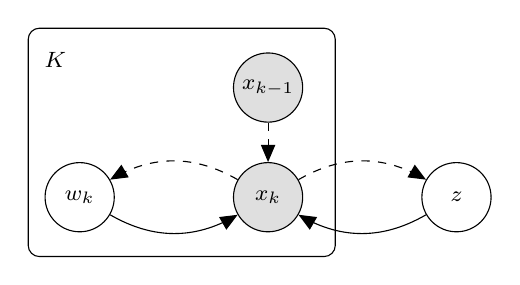
\begin{tikzpicture}[
  latent/.append style={
    minimum width=25pt,
    font=\footnotesize
  },
  plate caption/.append style={below right=0pt and 0pt of #1.north west},
]
\node[obs] (xk) {$x_k$};
\node[obs, above=.5cm of xk] (xkp) {$x_{k-1}$};
\node[latent, right=1.5cm of xk] (z) {$z$};
\node[latent, left=1.5cm of xk] (wk) {$w_k$};

\plate [inner sep=.3cm, xshift=0.1cm] {xw} {(wk)(xk)(xkp)} {$K$};
%\plate [inner sep=.5cm] {xwz} {(wk)(xk)(z)(xkp)} {$N$};

\path (wk) edge[bend right, ->] (xk);
\path (z) edge[bend left, ->] (xk);

\path (xk) edge[dashed, bend right, ->]  (wk);
\path (xk) edge[dashed, bend left, ->]  (z);
\path (xkp) edge[dashed, ->]  (xk);

\end{tikzpicture}

}
  \caption{%
  In the generative model (solid arrows), $K$ chunks $\{x_{k}\}$ (observed) share the same content~$z$, while having their own motion~$w_k$.
During inference (dashed arrows), the latent variables $z$ and~$w_k$ are inferred from each chunk, while each chunk~$x_k$ also depends on the previous one.
  }
  \label{fig:graphical_model}%
\end{figure}

Different from common frame-wise approaches, where~$w$ normally depend on previous frames, in the generative phase, we model all the motion representations $\{w_k\}$ as independent random variables.
This assumption simplifies the generation process since it lets us generate a particular chunk without having to consider the previous ones in the video.
A unique $z$ for all the chunks sets an implicit dependence of each chunk to the whole video in the inference phase of the model.

Being the chunks independent, the joint probability of the model is the product of the conditionals of each chunk and their latent variables, \ie,
\begin{equation}
p(x, w, z) = p(z)\prod_k p(x_{k} \given w_k, z)p(w_k).
\end{equation}
We model the generative process of a single chunk through a VAE~\cite{Kingma2013}, with content encoder $q_\phi(z \given x_{k})$, motion encoder $q_\gamma(w_k \given x_{k})$, and decoder $p_\theta(x_{k} \given w_k, z)$ with parameters ($\phi$, $\gamma$, $\theta$), updated to maximize of the evidence lower bound (ELBO) of the expected log-likelihood
\begin{align}
\argmax_{\phi, \gamma, \theta} \E_{\tilde{q}(x_{1:k})} \sum_k \Big\lbrace & \E_{q_\phi}\E_{q_\gamma} \left[\log p_\theta(x_k \given w_k, z) \right] \nonumber \\
& - \kl{q_\gamma(w_k \given x_k)}{p(w_k)} \nonumber \\
& - \kl{q_\phi(z \given x_k)}{p(z)} \Big\rbrace.
\label{eq:elbo_whole}
\end{align}
Fig.~\ref{fig:logp} shows the pipeline to calculate the ELBO~(\ref{eq:elbo_whole}).
We maximize the expected reconstruction loss over the two latent variables \wrt their distributions $q_\phi(z \given x_{k})$ and $q_\gamma(w_k \given x_{k})$ (first term), and minimize the Kullback-Leibler divergence between these distributions \wrt their priors.
We compute their expected value \wrt the empirical distribution of the chunks $\tilde{q}(x_{1:k}) = \prod_k q(x_{k} \given x_{k-1})$ that models a Markovian temporal relation between them.\footnote{We assume the first chunk to be distributed through $q(x_1 \given x_0) \equiv q(x_1)$ to simplify the notation.}
We approximate the chunk distribution through a sampling process on the videos, and model all prior distributions as standard Gaussians.
To generate a new video from the chunk posterior, we concatenate the expected values of the chunk posteriors, directly provided by the decoder.
See Appendix~\ref{sec:elbo} for further detail and proof of our formulation.

\begin{figure}[tb]%
  \centering%
  \resizebox{\linewidth}{!}{% !TeX spellcheck = en_US
\makeatletter%
\begin{tikzpicture}[
pics/named code/.style={code={\tikz@fig@mustbenamed%
  \begin{scope}[local bounding box/.expanded=\tikz@fig@name]#1\end{scope}%
}},
%pics/named code/.style={code={\tikz@fig@mustbenamed%
%    \node[inner sep=1pt, outer sep=1pt, anchor=center] (\tikz@fig@name) {\begin{tikzpicture}#1\end{tikzpicture}};%
%}},
% Encoder-Decoder pics
coder long height/.store in=\longheight,
coder long height=1,
coder short height/.store in=\shortheight,
coder short height=.5,
coder width/.store in=\width,
coder width=0.6,
coder fill/.store in=\coderfill,
coder text/.store in=\codertext,
coder label/.store in=\coderlabel,
latent label left/.store in=\latentlabelleft,
latent label right/.store in=\latentlabelright,
coder style hidden/.style={#1},
coder style hidden/.default={coder label=, coder text=white, coder fill=black,},
% note that pic should be centered at 0,0
pics/encoder tb/.style = {named code={%
  \tikzset{coder style hidden, #1}%
  \coordinate (-center) at (0, 0);
  \coordinate (-east) at (0,-\width/2);
  \coordinate (-west) at (0, \width/2);
  \coordinate (-north east) at (-\shortheight/2, -\width/2);
  \coordinate (-south east) at (\shortheight/2 , -\width/2);
  \coordinate (-north west) at (-\longheight/2 ,  \width/2);
  \coordinate (-south west) at (\longheight/2  ,  \width/2);
  \draw[fill=\coderfill] (-west) -- (-north west) -- (-north east) -- (-south east) -- (-south west) -- (-west);
  \node[text=\codertext, anchor=center] at (-center)  {\normalsize\coderlabel};%
}},
pics/encoder lr/.style = {named code={%
    \tikzset{coder style hidden, #1}%
    \coordinate (-center) at (0, 0);
    \coordinate (-west) at (-\width/2,0);
    \coordinate (-north west) at (-\width/2, \longheight/2);
    \coordinate (-north east) at (\width/2, \shortheight/2);
    \coordinate (-east) at (\width/2, 0);
    \coordinate (-south east) at (\width/2, -\shortheight/2);
    \coordinate (-south west) at (-\width/2, -\longheight/2);
    \draw[fill=\coderfill] (-west) -- (-north west) -- (-north east) -- (-south east) -- (-south west) -- (-west);
    \node[text=\codertext, anchor=center] at (-center)  {\coderlabel};%
}},
pics/decoder bt/.style = {named code={%
  \tikzset{coder style hidden, #1}%
  \coordinate (-center) at (0, 0);
  \coordinate (-east) at (0,  \width/2);
  \coordinate (-west) at (0, -\width/2);
  \coordinate (-north east) at (-\longheight/2 , \width/2);
  \coordinate (-south east) at ( \longheight/2 , \width/2);
  \coordinate (-north west) at (-\shortheight/2,-\width/2);
  \coordinate (-south west) at ( \shortheight/2,-\width/2);
  \draw[fill=\coderfill] (-west) -- (-north west) -- (-north east) -- (-south east) -- (-south west) -- (-west);
  \node[text=\codertext, anchor=center] at (-center)  {\normalsize\coderlabel};%
}},
pics/decoder rl/.style = {named code={%
  \tikzset{coder style hidden, #1}%
  \coordinate (-center) at (0, 0);
  \coordinate (-west) at (-\width/2,0);
  \coordinate (-north west) at (-\width/2, \shortheight/2);
  \coordinate (-north east) at (\width/2, \longheight/2);
  \coordinate (-east) at (\width/2, 0);
  \coordinate (-south east) at (\width/2, -\longheight/2);
  \coordinate (-south west) at (-\width/2, -\shortheight/2);
  \draw[fill=\coderfill] (-west) -- (-north west) -- (-north east) -- (-south east) -- (-south west) -- (-west);
  \node[text=\codertext, anchor=center] at (-center)  {\coderlabel};%
}},
chunk width/.store in=\wch,
chunk height/.store in=\hch,
chunk size/.store in=\sch,
chunk depth/.store in=\dch,
chunk fill/.store in=\chunkfill,
chunk text/.store in=\chunktext,
chunk label/.store in=\chunklabel,
chunk seq label/.store in=\chunkseqlabel,
chunk style/.style={#1},
chunk style/.default={chunk label=, chunk text=black, chunk fill=white,font=\tiny},
% note that pic should be centered at 0,0
pics/chunk/.style = {named code={%
  \tikzset{chunk style, #1}%
  \draw[fill=\chunkfill] (-\wch/2,-\hch/2) rectangle (\wch/2,\hch/2);
  %todo this part causes alignment issues
  \draw[fill=\chunkfill, rounded corners=0] (\wch/2,-\hch/2) -- (\wch/2+\dch,-\hch/2+\dch/2) -- (\wch/2+\dch,\hch/2+\dch/2) -- (\wch/2,\hch/2) -- (\wch/2,-\hch/2);
  \draw[fill=\chunkfill, rounded corners=0] (\wch/2,\hch/2) -- (\wch/2+\dch,\hch/2+\dch/2) -- (-\wch/2+\dch,\hch/2+\dch/2) -- (-\wch/2,\hch/2) -- (\wch/2,\hch/2);
  \node[text=\chunktext, anchor=center, inner sep=0pt, outer sep=0pt] at (0,0) {\chunklabel};%
}},
pics/chunk seq/.style = {named code={%
  \tikzset{chunk style, #1}%
  \pic[] (-1) at (-2*\sch,0) {chunk={chunk label=$\chunkseqlabel_{1}$, chunk width=\sch, chunk height=\sch}};%
  \pic[] (-2) at (-\sch,0) {chunk={chunk label=$\chunkseqlabel_{2}$, chunk width=\sch, chunk height=\sch}};%
  \pic[] (-dots) at (\sch/2,0) {chunk={chunk label=$\dots$, chunk width=2*\sch, chunk height=\sch}};%
  \pic[] (-n) at (2*\sch,0) {chunk={chunk label=$\chunkseqlabel_{O}$, chunk width=\sch, chunk height=\sch}};%
}},%
pics/chunk grid/.style = {named code={%
  \tikzset{chunk style, #1}%
  \pic[] (-n1) at (-2*\sch,-\sch) {chunk={chunk label={$\rho_{O,1}$}, chunk width=\sch, chunk height=\sch}};%
  \pic[] (-n2) at (-\sch,-\sch) {chunk={chunk label={$\rho_{O,2}$}, chunk width=\sch, chunk height=\sch}};%
  \pic[] at (\sch/2,-\sch) {chunk={chunk label=$\dots$, chunk width=2*\sch, chunk height=\sch}};%
  \pic[] (-nn) at (2*\sch,-\sch) {chunk={chunk label={$\rho_{O,O}$}, chunk width=\sch, chunk height=\sch}};%
  \pic[] at (-2*\sch,\sch/2) {chunk={chunk label=$\vdots$, chunk width=\sch, chunk height=2*\sch}};%
  \pic[] at (-\sch,\sch/2) {chunk={chunk label=$\vdots$, chunk width=\sch, chunk height=2*\sch}};%
  \pic[] at (\sch/2,\sch/2) {chunk={chunk label={$\rho_{i,j}$}, chunk width=2*\sch, chunk height=2*\sch}};%
  \pic[] at (2*\sch,\sch/2) {chunk={chunk label=$\vdots$, chunk width=\sch, chunk height=2*\sch}};%
  \pic[] (-21) at (-2*\sch,2*\sch) {chunk={chunk label={$\rho_{2,1}$}, chunk width=\sch, chunk height=\sch}};%
  \pic[] (-22) at (-\sch,2*\sch) {chunk={chunk label={$\rho_{2,2}$}, chunk width=\sch, chunk height=\sch}};%
  \pic[] at (\sch/2,2*\sch) {chunk={chunk label=$\dots$, chunk width=2*\sch, chunk height=\sch}};%
  \pic[] (-2n) at (2*\sch,2*\sch) {chunk={chunk label={$\rho_{2,O}$}, chunk width=\sch, chunk height=\sch}};%
  \pic[] (-11) at (-2*\sch,3*\sch) {chunk={chunk label={$\rho_{1,1}$}, chunk width=\sch, chunk height=\sch}};%
  \pic[] (-12) at (-\sch,3*\sch) {chunk={chunk label={$\rho_{1,2}$}, chunk width=\sch, chunk height=\sch}};%
  \pic[] at (\sch/2,3*\sch) {chunk={chunk label=$\dots$, chunk width=2*\sch, chunk height=\sch}};%
  \pic[] (-1n) at (2*\sch,3*\sch) {chunk={chunk label={$\rho_{1,O}$}, chunk width=\sch, chunk height=\sch}};%
}},%
block heigth/.store in=\hb,
block fill/.store in=\blockfill,
block text/.store in=\blocktext,
block label/.store in=\blocklabel,
block style/.style={#1},
block style/.default={block label=, block text=black, block fill=white,},
comp heigth/.store in=\ch,
comp label/.store in=\complabel,
mult heigth/.store in=\mh,
pics/z block/.style = {named code={%
  \tikzset{block style, #1}%
  \draw[fill=\blockfill] (-\hb/3.236,-\hb/2) rectangle (\hb/3.236,\hb/2);
  \node[text=\blocktext, anchor=center] at (0,0.4*\hb) {\tiny $\blocklabel_1$};
  \draw[] (-\hb/3.236,0.3*\hb) -- (\hb/3.236,0.3*\hb);
  \node[text=\blocktext, anchor=center] at (0,0.2*\hb) {\tiny $\blocklabel_2$};
  \draw[] (-\hb/3.236,0.1*\hb) -- (\hb/3.236,0.1*\hb);
  \node[text=\blocktext, anchor=center] at (0,-0.05*\hb) {\tiny $\vdots$};
  \draw[] (-\hb/3.236,-0.3*\hb) -- (\hb/3.236,-0.3*\hb);
  \node[text=\blocktext, anchor=center] at (0,-0.4*\hb) {\tiny $\blocklabel_O$};
}},
pics/z block comp/.style = {named code={%
  \tikzset{block style, #1}%
  \draw[fill=\blockfill] (-\ch/1.618,-\ch/2) rectangle (0,\ch/2);
  \pic[] at (\ch/3.236,0) {z block={block heigth=\ch, block label=w}};
  \node[text=\blocktext, anchor=center] at (-\ch/3.236,0) {\tiny \complabel};
}},
pics/z block mult/.style = {named code={%
  \tikzset{block style, #1}%
  \pic[] at (0,0) {z block comp={comp heigth=\mh, comp label=$z_1$}};
  \draw[fill=\blockfill] (-\mh/1.618,-\mh*.5) rectangle (\mh/1.618,-\mh*.9);
  \node[text=\blocktext, anchor=center] at (0,-\mh*.65) {$\vdots$};
  \pic[] at (0,-\mh*1.4) {z block comp={comp heigth=\mh, comp label=$z_O$}};
}},
loss/.style={
  shorten <=2.5pt, 
  shorten > = 2.5pt,
  <->,
  >=latex,
  draw=#1,
  text=#1,
  my node/.style={%
    text width=20pt,
    inner sep=1pt,
    text centered,
    circle,
    rounded corners,
    fill=white, 
    draw,
  },
  every node/.style={my node},
  my node,
  fill=none,
},
loss/.default=black,
font=\tiny,
flow/.style={rounded corners, -{latex}},
ll/.style={-{latex}, dashed, blue!80, line width = 1},
lr/.style={-{latex}, dashed, red!80,  line width = 0.75},
lrbl/.style={-{latex}, lr, bend left=60, looseness=.6},
lrbr/.style={-{latex}, lr, bend right=60, looseness=0.6},
rr/.style={-{latex}, dashed, blue!40!green!80,  line width = 0.75},
% for the matrix (makes the line thiner)
table/.style={
  row sep=-\pgflinewidth,
  column sep=-\pgflinewidth,
  nodes={draw, anchor=center},
  nodes={inner sep=0pt, outer sep=0pt,},
  execute at empty cell={\node[draw=none]{};},
},
% make all nodes the minium same size
every node/.style={
  minimum height=1.8em, minimum width=1.8em,
},
% tight style for labels (removes all white space around them)
tight/.style={
  outer sep=0pt, inner sep=0pt, minimum width=1em, minimum height=1em,
},
node distance=.5,
]
\makeatother

%% Original video
\matrix[table, matrix of math nodes] (x) {
  x_1 & x_2 & \dots & x_O \\
};

%% Encoders
\pic[right = 1 of x] (ea) {encoder lr={coder label={$q_\phi$}}};
\pic[below= .75 of ea] (em) {encoder lr={coder label={$q_\gamma$}}};


%% Latent vectors
\matrix[matrix of math nodes, right=of ea, nodes={draw, anchor=center}] (latz) {
 z_1 & z_2 & \dots & z_O \\
};
\matrix[matrix of math nodes, right=of em, nodes={draw, anchor=center}] (latw) {
  w_1 & w_2 & \dots & w_O \\
};

%% Combined latent space
\matrix[table, matrix of math nodes, nodes in empty cells, below=.125 of latw, nodes={minimum height=1em}] (lat) {
  & w_1 \\
  & \dots \\
  & w_O \\
  & \\
  & w_1 \\
  & \dots \\
  & w_O \\
};
\node[draw, fill=white, fit=(lat-1-1)(lat-3-1), inner sep=0pt, outer sep=0pt] {$z_1$};
\node[draw, fill=white, fit=(lat-4-1)(lat-4-2), inner sep=0pt, outer sep=0pt, minimum height=1em] {$\dots$};
\node[draw, fill=white, fit=(lat-5-1)(lat-7-1), inner sep=0pt, outer sep=0pt] {$z_O$};

%% Grid of parameters
\matrix[matrix of math nodes, table, nodes in empty cells] (grid) at (x |- lat) {
  \rho_{1,1} & \rho_{1,2} & \dots & \rho_{1,O} \\
  \rho_{2,1} & \rho_{2,2} & \dots & \rho_{2,O} \\
  \rvdots & \rvdots & \rho_{j,k} & \rvdots \\
  \rho_{O,1} & \rho_{O,2} & \dots & \rho_{O,O} \\
};

%% Generated video
\matrix[table, matrix of math nodes, below=of grid] (x') {
  \hat{x}_1 & \hat{x}_2 & \dots & \hat{x}_O \\
};

%% Priors
\node[loss=black, right=1 of latz] (pz) {$p(z)$};
\node[loss=black, right=1 of latw] (pw) {$p(w_k)$};

%% Decoder
\pic[] (d) at (em |- grid) {decoder rl={coder label={$p_\theta$}}};


%% Flow
\draw[flow] (x.east) -- (ea.west);
\draw[flow] (x.east) -| ($(x.east |- em.west)!.5!(em.west)$) -- (em.west);

\draw[flow] (ea) -- (latz);
\draw[flow] (em) -- (latw);

\draw[flow] ($(latz.east)+(0,-.25em)$) -| (lat -| {$(latz.east)!.5!(pz.west)$}) -- (lat);
\draw[flow] ($(latw.east)+(0,-.25em)$) -| (lat -| {$(latw.east)!.5!(pw.west)$}) -- (lat);

\draw[flow] (lat) -- (d);
\draw[flow] (d) -- (grid);

\draw[ll] (latz) --node[circle, above=2.5pt, blue, tight] {\small $\mathcal{L}_a$} (pz);
\draw[ll] (latw) --node[circle, above=2.5pt, blue, fill=white, tight] {\small $\mathcal{L}_m$} (pw);

%% Loss reconstruction
\path (grid-1-1.west) edge[lrbl] (x-1-1.south);
\path (grid-2-1.west) edge[lrbl] (x-1-1.south);
\path (grid-4-1.west) edge[lrbl] (x-1-1.south);

\path (grid-1-4.east) edge[lrbr] (x-1-4.south);
\path (grid-2-4.east) edge[lrbr] (x-1-4.south);
\path (grid-4-4.east) edge[lrbr] node[circle, fill=white, above left, xshift=0pt, yshift=5pt, tight] {\small $\mathcal{L}_r$} (x-1-4.south);


%% Sampling
\path (grid-4-1.south) edge[rr] (x'-1-1.north);
\path (grid-4-2.south) edge[rr] (x'-1-2.north);
\path (grid-4-4.south) edge[rr] (x'-1-4.north);

%% Labels
\node[above=-7pt of x.north west, anchor=south west] {\scriptsize Input video};
\node[above=-0pt of grid] {\scriptsize Chunk posteriors'};
\node[above=-7pt of grid] {\scriptsize parameters};
\node[below=-7pt of x'.south west, anchor=north west] {\scriptsize Reconstructed video};
\node[below=-5pt of lat] {\scriptsize Combined latent representations};

\node[below=0pt of em] {\scriptsize Encoders};
\node[below=0pt of d] {\scriptsize Decoder};

\node[above=-7pt of latz.north west, anchor=south west] {\scriptsize Appearance representations};
\node[above=-7pt of latw.north west, anchor=south west] {\scriptsize Motion representations};

\node[blue!40!green, fill=white, tight] at ($(grid.south)!.5!(x'.north)$) {\scriptsize Sampling};

\end{tikzpicture}%
\makeatother%}
 \caption{%
  We feed consecutive chunks $\{x_k\}_{k=1}^O$ to the encoders $q_\phi$ and $q_\gamma$, yielding their representations, $\{w_k\}_{k=1}^O$ and $\{z_j\}_{j=1}^O$.
  We concatenate all combinations of $z_j$'s and $w_k$'s, and decode them to obtain the p.d.f.\ parameters $\rho_{j,k}$ for the $k$-th chunk posteriors $p_\theta(x_k \given w_k, z_j)$.
  Every posterior from $w_k$ must generate $x_k$.
  We maximize the log-likelihood of each chunk under the corresponding set of posteriors.
  Chunk posteriors \textcolor{red}{relate} with the original chunks through $\mathcal{L}_r$.
  The latent prior distributions \textcolor{blue}{relate} through $\mathcal{L}_a$ and $\mathcal{L}_m$.
  We \textcolor{blue!40!green}{sample} from the chunk posterior by applying the Sigmoid function to the output of the decoder.
  }
  \label{fig:logp}%
\end{figure}

Our architecture consists of two encoders $q_\phi(z \given x_{k})$ and $q_\gamma(w_k \given x_{k})$, and one decoder $p_\theta(x_{k})$\@.
All of them have five 3D-convolutional layers, with Batchnorm and ReLU activations.
The number of filters in the hidden layers of the decoder is double the number of filters in the encoders.

\subsection{Inter-Chunk Consistency}
\label{sec:inter-chunk-consistency}

As shown in Equation~\ref{eq:elbo_whole}, we can train a VAE to independently reconstruct chunks.
However, the independence assumption at generation time may cause the videos to not be smoothly rendered between chunks.
To solve this issue, we force our model to yield a unique content representation~$z$, regardless of the chunk from which it is inferred.

We part from the assumption that content is constant throughout the video, and so does its latent representation $z \sim q_\phi(z \given x_{k})$---\cf Section~\ref{sec:modeling}.
To force our model to learn this constraint, we train it to maximize $\log p_\theta(x_{k} \given w_k,z_j)$ for every~$j$, \ie, maximize the log-likelihood of a chunk $x_{k}$ given its own motion~$w_k$ and any~$z_j$ content representation---\cf Fig.~\ref{fig:logp}.
We extend the $\log p(x_{k} \given  w_k, z)$ term~(\ref{eq:elbo_whole}) to fulfill this constraint.
So our final reconstruction loss is
\begin{equation}
\label{eq:logp_x}
\mathcal{L}_{r}(\theta, \phi,\gamma) = \sum_{k=1}^O\sum_{j=1}^O \left[\log p_\theta(x_{k} \given w_k,z_j)\right],
\end{equation}
where $z_j \sim q_\phi(z \given x_{j})$, $w_k \sim q_\gamma(w_k \given x_{k})$, and $O$ is defined as the \textit{order of the model} that restricts the number of chunks used to calculate the loss.
As Fig.~\ref{fig:logp} shows, the decoder outputs the distribution parameters $\rho_{j,k}$ of each chunk likelihood $p_\theta(x_{k} \given w_k,z_j)$, used in $\mathcal{L}_{r}$.
Due to its combinatory nature, it is impractical to apply $\mathcal{L}_r$ to all the chunks.
Hence, for each forward pass, we consider only a sequence of $O \le K$ consecutive chunks of $x$, starting at a random frame.

The second and third terms of the expected log-likelihood~(\ref{eq:elbo_whole}) correspond to the regularization terms of the motion and content distributions, respectively.
That is, we compute
\begin{align}
  \label{eq:lm}
  \mathcal{L}_{m}(\gamma)&= -\sum_{k=1}^O \kl{q_\gamma(w_k \given x_k)}{p(w_k)}, \text{ and} \\
  \label{eq:la}
  \mathcal{L}_{a}(\phi)&= -\sum_{k=1}^O \kl{q_\phi(z \given x_k)}{p(z)},
\end{align}
on $O$ consecutive chunks instead of the whole video---\cf Fig.~\ref{fig:logp}.

Unlike other variational inference methods of grouped observations~\cite{Locatello2020,Mathieu2016,Bouchacourt2018,Hosoya2019}, we opted for the extended log-probability term~(\ref{eq:logp_x}), considering different combinations of appearance features, to yield stronger gradients for chunk-consistency, instead of averaging the shared representations in the group.

\subsection{Blind Reenactment Loss}
\label{sec:brl}

Our proposed Blind Reenactment Loss (BRL) loss increases the likelihood $\log p(x_{k} \given w_k, z)$ of our ELBO given any encoded chunks.
It aims at leveraging content-motion disentanglement by doing VR between a source video~$S$ and a driving video~$D$.
The motion representation of $S$ is replaced by the one of $D$, to reconstruct a reenacted video with the object of interest from $S$ moving like the one in $D$.
This translation can be achieved uniquely if the content and motion representations of both videos are disentangled.
The main difficulty is that, in principle, we would need to train our model with ground-truth reenacted videos.
However, we opt for self-supervised training and take advantage of our chunk-based approach.

Consider two chunks $s_i$ and~$s_j$ from $S$, and one chunk $d_l$ from $D$.
Assuming constant content throughout the video, if we independently reenact $s_i$ and~$s_j$ \wrt $d_l$, the two reconstructed chunks must be the same since $s_i$ and $s_j$ have the same content.
To achieve this objective, we force the corresponding chunk posteriors $p(x_{k} \given w_k, z)$ to be equivalent, \ie, $p(x \given w_l^d, z_j^s) \equiv p(x \given w_l^d, z_i^s)$, where $z_i^s \sim q(z \given s_i)$, $z_j^s \sim q(z \given s_j)$, and $w_l^d \sim q(w_k \given d_l)$, by minimizing the KL divergence between every two posteriors that fit the described case.
Let
\begin{align}
  \label{eq:brl}
\mathcal{L}_b & (\theta,\phi,\gamma) = \nonumber \\
& -\sum_{l=1}^O\sum_{j=1}^O\sum_{i=1}^O \operatorname{SKL} \Big(p_\theta(x \given  w_l^d,z_j^s) \;\big\| p_\theta(x \given w_l^d,z_i^s) \Big).
\end{align}
be our BRL, where $\skl{P}{Q}= \frac{1}{2}(\kl{P}{Q} + \kl{Q}{P})$ is a symmetrical operator.
This loss involves two empirical distributions of unobservable samples, so we are not aware, at training time, of whether the sampled videos are correctly reenacted.
If there is disentanglement, posteriors sharing the same motion of $D$ and \textit{any} content of $S$ must be equivalent, regardless of their samples.

The BRL must be optimized along with $\mathcal{L}_r$~(\ref{eq:logp_x}) to prevent posterior collapse.
Notice that, if $O = 1$, then $j=i=1$ and $\mathcal{L}_b=0$, so this objective can only be optimized for $O \geq 2$.

\subsection{General Loss Function}

We define the general objective to be maximized as
\begin{equation}
\mathcal{L} = \mathcal{L}_r + \lambda\mathcal{L}_b + \beta(\mathcal{L}_a + \mathcal{L}_m),
\end{equation}
where $\beta$ comes from $\beta$-VAE by \cite{Higgins2017}, and $\lambda$ weights $\mathcal{L}_b$\@.
Each element in the batch is conformed by a sequence of $O$ chunks, so $\mathcal{L}$ can be calculated independently for every element.

\section{Experiments}
\label{sec:experiments}

\begin{table*}[tb]
  \caption{Performance for content-motion disentanglement and data realism. (*\,$c=1$)}
  \label{tab:baselines}
  \scriptsize
  \centering
  \resizebox{\linewidth}{!}{%
  \begin{tabular}{cSSSSS[table-format=3.2(4)]cSSSSS[table-format=3.2(4)]}
    \toprule
    &   {FVAE $\uparrow$} & {MIG $\uparrow$} & {SAP $\uparrow$} & {SSIM $\uparrow$} & {FID $\downarrow$}
    & & {FVAE $\uparrow$} & {MIG $\uparrow$} & {SAP $\uparrow$} & {SSIM $\uparrow$} & {FID $\downarrow$} \\
    \cmidrule{2-6} \cmidrule{8-12}
    & \multicolumn{5}{c}{3dShapes} & & \multicolumn{5}{c}{LPC} \\
    \cmidrule{2-6} \cmidrule{8-12}
    $\beta$-TCVAE & .50(2) & \bf .01(1) &     .11(8)  &     .53(10) &    140.25(5113) & &     .81(3) &     .02(02) &     .00(00) &     .64(1) &     80.27(317) \\
    dis-VAE       & .50(0) &     .00(0) &     .08(6)  &     .40(3)  & \bf 71.24(1235) & &     .92(2) &     .02(02) &     .01(01) &     .78(1) &     71.70(176) \\
    SVG-LP        & .50(0) & \bf .01(0) &     .03(02) &     .54(5)  &    136.00(8112) & &     .63(2) &     .00(00) &     .00(00) & \bf .79(2) &     62.75(987) \\
    MTC-VAE       & .50(2) & \bf .01(0) & \bf .41(14) &     .67(6)  &    119.47(5100) & & \bf .93(6) & \bf .11(11) & \bf .60(40) &     .67(1) & \bf 41.72(331) \\
    MTC-VAE*      & .50(1) & \bf .01(0) &     .39(11) & \bf .73(2)  &    100.80(4682) & &     .86(1) &     .00(00) &     .11(03) &     .67(1) &     42.59(409) \\
    \cmidrule{2-6} \cmidrule{8-12}
    & \multicolumn{5}{c}{CK+} & & \multicolumn{5}{c}{MMNIST} \\
    \cmidrule{2-6} \cmidrule{8-12}
    $\beta$-TCVAE &     .79(5) & \bf .03(2) &     .06(4)  &     .50(7)  &    116.74(2470) & &     .66(7) &     .04(4) &     .04(4)  & \bf .71(3) &     152.56(1693) \\
    dis-VAE       &     .71(2) &     .01(1) &     .04(2)  &     .61(5)  &     71.48(309)  & &     .64(4) &     .02(2) &     .03(2)  &     .70(2) &     149.43(973) \\
    SVG-LP        &     .70(6) &     .02(1) &     .04(2)  &     .02(0)  & \bf 38.79(1763) & &     .52(1) &     .01(0) &     .02(2)  &     .58(2) &     179.08(5049) \\
    MTC-VAE       & \bf .86(4) &     .02(1) & \bf .13(5)  &     .66(12) &     63.13(2250) & & \bf .95(4) & \bf .11(7) & \bf .10(5)  &     .68(1) & \bf 102.11(99) \\
    MTC-VAE*      &     .85(2) & \bf .03(1) &     .05(2)  & \bf .68(13) &     76.16(1937) & &     .91(4) &     .09(5) &     .09(4)  &     .69(1) &     186.25(2355) \\
    \cmidrule{2-6} \cmidrule{8-12}
    & \multicolumn{5}{c}{dSprites} & & \multicolumn{5}{c}{MUG} \\
    \cmidrule{2-6} \cmidrule{8-12}
    $\beta$-TCVAE &     .57(3) &     .00(0) &     .04(1) & \bf .79(3) &     79.34(618) & &     .74(5) & \bf .05(4) &     .23(03) &     .51(01) &     44.78(332) \\
    dis-VAE       &     .70(2) &     .01(0) &     .01(0) & \bf .79(0) &     97.07(173) & & \bf .76(3) &     .01(1) &     .11(03) & \bf .78(01) &     62.84(345) \\
    SVG-LP        &     .61(5) &     .00(0) &     .00(0) & \bf .79(2) &     98.14(920) & &     .64(4) &     .02(1) &     .38(04) &     .50(15) &    101.59(3700) \\
    MTC-VAE       &     .91(2) & \bf .04(1) & \bf .10(1) &     .78(0) & \bf 57.18(643) & &     .72(4) &     .01(1) &     .73(05) &     .63(02) & \bf 28.79(115) \\
    MTC-VAE*      & \bf .92(1) &     .02(2) &     .01(0) &     .77(1) &    105.79(586) & &     .70(9) &     .04(2) & \bf .76(10) &     .66(06) &     43.86(1315) \\
    \bottomrule
  \end{tabular}}

\end{table*}

We evaluated MTC-VAE in DRL, VR, and downstream tasks.
Although MTC-VAE does not require labels in training time, we used labels to asses disentanglement, and to split the training and testing datasets.
We detail the implementation of the model and the experimental setup in Appendix~\ref{sec:implementation}.

\textbf{Datasets.}
(i)~Cohn-Kanade (CK+) facial dataset~\cite{Kanade2000, Lucey2010}, (ii)~Liberated Pixel Cup (LPC) sprites, (iii)~Moving MNIST (MMNIST)~\cite{Srivastava2015}, (iv)~Deepmind's dSprites, (v)~Deepmind's 3dShapes, and (vi)~Multimedia Understanding Group (MUG) facial dataset~\cite{Aifanti2010}.
We generated videos from the images of dSprites and 3dShapes, forming sequences of objects moving in linear and curved trajectories, or changing their perspective.
Each dataset contains \num{10000} videos, except for CK+ (\num{320}), LPC (\num{200000}), and MUG (\num{700}).
We report the average model performance in a $5$-fold cross-validation setup ($80\%$ for training and $20\%$ for testing).
Appendix~\ref{sec:data} provides further detail about the datasets, as well as the factors of variation.

\textbf{Baselines.}
We compared our method against the Disentangled Sequential Autoencoder (dis-VAE) \cite{Li2018}, SVG-LP \cite{Denton2018}, and $\beta$-TCVAE \cite{Chen2018dr}.
The first two are frame-wise approaches that disentangle time-dependent from time-independent factors.
Although SVG-LP namely disentangles deterministic from stochastic features, they force the deterministic features to remain constant, while the stochastic ones change from frame to frame, like a content-motion modeling.
$\beta$-TCVAE is an unsupervised disentanglement model, tested so far on images, so we extended it to 3D-CNNs to support chunks.

\textbf{Hyper-parameters.}
After a hyper-parameter search in the models (see details in Appendix~\ref{sec:implementation}), we tuned the $\beta$ parameter and the latent space size.
For dSprites, LPC and MMNIST, $\beta = 1$, and $\beta = 5$ for the other datasets.
Regarding the latent space dimensionality (where each dimension is a \textit{latent unit}), $\text{dim}(z)=14$, $\text{dim}(w_k)=7$ for CK+, LPC, and MUG, $\text{dim}(z)=12$, $\text{dim}(w_k)=6$ for 3dShapes, $\text{dim}(z)=12$, $\text{dim}(w_k)=4$ for dSprites, and $\text{dim}(z)=8$, $\text{dim}(w_k)=4$ for MMNIST.
We performed ablation studies on $\lambda$, $c$, $O$, and $\beta$ (\cf Section~\ref{sec:ablation} and Appendix~\ref{sec:detailed_results}).

\subsection{Content-Motion Disentanglement}
\label{sec:experiments_disentanglement}

We obtained the latent representations from the trained models for the test set and, using ground-truth labels, we calculated the Mutual Information Gap (MIG)~\cite{Chen2018dr}, the FactorVAE (FVAE) disentanglement metric~\cite{Kim2018}, and the Separated Attribute Predictability Score (SAP)~\cite{Kumar2018}.

Assessing disentanglement quality is narrowly application-related~\cite{Eastwood2018,Ridgeway2018}.
We adhere to the criteria defined by \textcite{Ridgeway2018}, by which we may evaluate disentanglement based on either \emph{modularity} (\ie, each unit contains information of at most one factor), \emph{compactness} (\ie, each factor is ideally encoded by at most one unit) or \emph{explicitness} (\ie, each factor is easily recovered from its code).

Since our objective is to encode two factors of variation (content and motion) in various latent units, our main interest is modularity.
Compactness, although desirable, is expected to not be fulfilled, as content and motion are complex factors that can barely be represented in few latent units.
Explicitness is important to estimate the effectiveness of disentangled representations for downstream tasks, like classification.

MIG and SAP heavily penalize representations that are not compact, by depending on the mean difference between the first and second most predictive/informative units.
Hence, FVAE is the metric that interests us the most, as it measures both modularity and explicitness.
We report results on MIG and SAP for completeness since, besides assessing compactness, to some extent, MIG also assesses modularity, and SAP, explicitness.

For $\beta$-TCVAE and MTC-VAE, we split every test video into chunks and calculated one latent vector per chunk.
For dis-VAE and SVG-LP, we obtained one vector per frame.
We aggregated the multiple factors, provided in 3dShapes, dSprites, and LPC, into two categories: time-dependent and time-independent, yielding two factors, to reduce the risk of over-estimation of disentanglement performance, due to pairs of disentangled factors while the rest are entangled.

Table~\ref{tab:baselines} shows the performance of the models on the content-motion disentanglement.
We included the results obtained for the frame-wise version of MTC-VAE (\ie, $c=1$) to compare against dis-VAE and SVG-LP\@.
Both the chunk and frame versions of MTC-VAE are the ones with the best disentanglement performance, followed by $\beta$-TCVAE\@ and dis-VAE.
It is remarkable that SVG-LP uses skip connections from the encoder to the decoder, so most of the appearance information is not in the latent representation.
This is reflected in the fact that it attained the poorest performance.
In general, the chunk version of MTC-VAE outperforms the frame version.

\begin{table}[tb]
\caption{Multi-factor disentanglement. (*\,$c=1$)}
\label{tab:mf}
\scriptsize
\centering
\begin{tabular}{crSSS}
\toprule
 & & {FVAE $\uparrow$} & {MIG $\uparrow$} & {SAP $\uparrow$} \\
\midrule
\multirow{5}{*}{3dShapes}
& $\beta$-TCVAE &     .21(3) &     .07(4) &     .03(2) \\
& dis-VAE       &     .19(1) &     .03(1) &     .01(1) \\
& SVG-LP        &     .18(1) &     .02(1) &     .01(0) \\
& MTC-VAE       &     .27(5) & \bf .19(7) & \bf .08(3) \\
& MTC-VAE*      & \bf .31(2) &     .14(5) &     .05(2) \\
\midrule
\multirow{5}{*}{dSprites}
& $\beta$-TCVAE &     .28(1) &     .02(1) &     .01(0) \\
& dis-VAE       &     .28(0) &     .02(1) &     .01(0) \\
& SVG-LP        &     .29(0) &     .00(0) &     .00(0) \\
& MTC-VAE       & \bf .33(2) & \bf .11(1) & \bf .02(0) \\
& MTC-VAE*      &     .29(1) &     .07(2) &     .01(0) \\
\midrule
\multirow{5}{*}{LPC}
& $\beta$-TCVAE &     .32(7) &     .16(9) &     .03(1) \\
& dis-VAE       &     .22(1) &     .04(1) &     .06(5) \\
& SVG-LP        &     .17(0) &     .01(0) &     .01(1) \\
& MTC-VAE       &     .41(7) & \bf .21(5) & \bf .89(1) \\
& MTC-VAE*      & \bf .43(6) &     .18(3) & \bf .89(0) \\
\bottomrule
\end{tabular}
\end{table}

\begin{figure*}[tb]
\centering
  \scriptsize
  \setlength{\subfigsz}{.32\linewidth}
  \setlength\tabcolsep{1.5pt}
  \begin{tabular}{cccccc}
    Source & Driving & Source & Driving & Source & Driving \\
    \boximg{.15}{MUG_s.png} &
    \boximg{.75}{MUG_d.png} &
    \boximg{.15}{LPC_s.png} &
    \boximg{.9}{LPC_d.png} &
    \boximg{.15}{dSprites_s.png} &
    \boximg{.75}{dSprites_d.png} \\
    $\beta$-TCVAE & \boximg{.75}{MUG_betaTC_p10000102.png} &
    $\beta$-TCVAE & \boximg{.9}{LPC_betaTC_p10000054.png} &
    $\beta$-TCVAE & \boximg{.75}{dSprites_betaTC_p10000002.png} \\
    dis-VAE & \boximg{.75}{MUG_dis_p10000102.png} &
    dis-VAE & \boximg{.9}{LPC_dis_p10000054.png} &
    dis-VAE & \boximg{.75}{dSprites_dis_p10000002.png} \\
    SVG-LP  & \boximg{.75}{MUG_SVG_p10000102.png} &
    SVG-LP  & \boximg{.9}{LPC_SVG_p10000054.png} &
    SVG-LP  & \boximg{.75}{dSprites_SVG_p10000002.png} \\
    MTC-VAE & \boximg{.75}{MUG_MTC_p10000102.png} &
    MTC-VAE & \boximg{.9}{LPC_MTC_p10000054.png} &
    MTC-VAE & \boximg{.75}{dSprites_MTC_p10000002.png}
  \end{tabular}
\caption{
  Reenactment results.  Each set shows the reenacted video of each method with the appearance of \textit{source} and the motion of \textit{driving}.
}
\label{fig:comparison}
\end{figure*}

Although MTC-VAE is trained for motion-content disentanglement, we can argue that this task can be used as a step towards multi-factor disentanglement.
To show our point, we calculated MIG, FVAE, and SAP considering all the factors of variation provided in the datasets' metadata.
Table~\ref{tab:mf} shows the results for 3dShapes, dSprites, and LPC since the others only provide motion-content labels.
In all cases, MTC-VAE (both frame and chunk versions) significantly outperforms the baselines.
The second best method was $\beta$-TCVAE, which is expected since it has been already tested on multi-factor disentanglement for images.
Table~\ref{tab:mf} demonstrates that multi-factor disentanglement is a significantly harder task, but it is remarkable that MTC-VAE features are more disentangled than the others, even when the model was not trained for this specific task.
We provide a list and a description of the factors of variation considered for each dataset in Appendix~\ref{sec:implementation}.

\subsection{Video Reenactment}
\label{sec:reenactment}

\begin{figure*}[tb]
\resizebox{\linewidth}{!}{% !TeX root=../paper.tex
\pgfplotstableread{
c 3dShapesFID 3dShapesFVAE 3dShapesMIG 3dShapesSAP 3dShapesSSIM CKFID CKFVAE CKMIG CKSAP CKSSIM dSpritesFID dSpritesFVAE dSpritesMIG dSpritesSAP dSpritesSSIM LPCFID LPCFVAE LPCMIG LPCSAP LPCSSIM MMNISTFID MMNISTFVAE MMNISTMIG MMNISTSAP MMNISTSSIM MUGFID MUGFVAE MUGMIG MUGSAP MUGSSIM AvgFID AvgFVAE AvgMIG AvgSAP AvgSSIM StdFID StdFVAE StdMIG StdSAP StdSSIM
1 100.8 .5 .01 .39 .73 76.16 .85 .03 .05 .68 105.79 .92 .02 .01 .77 42.59 .86 .00 .11 .67 186.25 .91 .09 .09 .69 43.86 .7 .04 .76 .66 92.58 .79 .03 .24 .70 53.21 .16 .03 .29 .04 
3 114.23 .51 .01 .41 .73 70.56 .87 .03 .11 .67 70.41 .87 .02 .06 .78 41.72 .93 .11 .60 .67 96.04 .95 .08 .09 .68 37.62 .73 .03 .7 .62 71.76 .81 .05 .33 .69 29.88 .17 .04 .28 .06 
5 119.47 .5 .01 .41 .67 63.13 .86 .02 .13 .66 68.48 .82 .03 .06 .78 84.87 .87 .00 .17 .66 102.11 .95 .07 .1 .68 37.08 .73 .01 .69 .62 79.19 .79 .02 .26 .68 29.41 .16 .03 .24 .05 
7 117.88 .48 .01 .32 .62 63.03 .85 .02 .12 .62 71.17 .79 .02 .05 .78 76.92 .87 .00 .16 .67 95.69 .92 .06 .09 .68 37.36 .72 .01 .72 .62 77.01 .77 .02 .24 .67 27.64 .16 .02 .25 .06 
9 124.43 .51 .01 .33 .58 60.56 .81 .03 .11 .61 72.77 .76 .03 .10 .78 53.57 .89 .01 .19 .67 116.05 .91 .1 .12 .68 37.56 .72 .02 .7 .61 77.49 .77 .03 .26 .66 35.12 .15 .03 .23 .07 
}\datatable

\pgfplotsset{cycle list/Dark2-6}

\begin{tikzpicture}[
  curve/.style={
    mark=*, mark size=1pt, smooth, thick
  },
  avg/.style = {
    curve, 
    draw=black!80, 
    opacity=0.75,
  },
  std/.style={
    fill=black!80, 
    opacity=0.15,
  },
  y double precision/.style = {
    /pgfplots/y tick label style={
      /pgf/number format/fixed,
      /pgf/number format/fixed zerofill,
      /pgf/number format/precision=2,
    },
  },
]
\begin{groupplot}[
  group style={
    group size=5 by 1, 
    horizontal sep=1cm,
  }, 
  cycle list/Dark2-6,
  xtick={1, 3, 5, 7, 9}, 
  xmin=0, xmax=10, 
  height=6cm, width=6cm,
  % ymin=0, ymax=1.0,
]

\nextgroupplot[
    title={FVAE $\uparrow$},
    ytick={0.4,0.5,...,1},
]

\foreach \c in {3dShapes, CK, dSprites, LPC, MMNIST, MUG} 
    \addplot+[curve] table[x=c,y=\c FVAE] from \datatable;

% draw avg
\addplot [avg] table[x=c,y=AvgFVAE] from \datatable;
% define error fill functions
\addplot [name path=upper, draw=none] table[x=c,y expr=\thisrow{AvgFVAE}+\thisrow{StdFVAE}] from \datatable;
\addplot [name path=lower, draw=none] table[x=c,y expr=\thisrow{AvgFVAE}-\thisrow{StdFVAE}] from \datatable;
% draw error
\addplot [std] fill between[of=upper and lower];

\nextgroupplot[
    title={MIG $\uparrow$},
    y double precision,
    ytick={0, 0.03,..., 0.12}, 
    % yticklabels={},
]

\foreach \c in {3dShapes, CK, dSprites, LPC, MMNIST, MUG} 
    \addplot+[curve] table[x=c,y=\c MIG] from \datatable;

% draw avg
\addplot [avg] table[x=c,y=AvgMIG] from \datatable;
% define error fill functions
\addplot [name path=upper, draw=none] table[x=c,y expr=\thisrow{AvgMIG}+\thisrow{StdMIG}] from \datatable;
\addplot [name path=lower, draw=none] table[x=c,y expr=\thisrow{AvgMIG}-\thisrow{StdMIG}] from \datatable;
% draw error
\addplot [std] fill between[of=upper and lower];

\nextgroupplot[
    title={SAP $\uparrow$},
    legend style={at={(.5,-.2)},anchor=center},
    % legend cell align={left},
    legend style={
      legend columns=7,
      draw=gray,
    },
    % xlabel={Chunk size ($c$)},
]

\legend{3dShapes, CK, dSprites, LPC, MMNIST, MUG, Avg.}

\foreach \c in {3dShapes, CK, dSprites, LPC, MMNIST, MUG} 
    \addplot+[curve] table[x=c,y=\c SAP] from \datatable;

% draw avg
\addplot [avg] table[x=c,y=AvgSAP] from \datatable;
% define error fill functions
\addplot [name path=upper, draw=none] table[x=c,y expr=\thisrow{AvgSAP}+\thisrow{StdSAP}] from \datatable;
\addplot [name path=lower, draw=none] table[x=c,y expr=\thisrow{AvgSAP}-\thisrow{StdSAP}] from \datatable;
% draw error
\addplot [std] fill between[of=upper and lower];

\nextgroupplot[
    title={SSIM $\uparrow$},
    y double precision,
    ytick={0.6,.65,...,0.8},
    % yticklabels={},
]

\foreach \c in {3dShapes, CK, dSprites, LPC, MMNIST, MUG} 
  \addplot+[curve] table[x=c,y=\c SSIM] from \datatable;

% draw avg
\addplot [avg] table[x=c,y=AvgSSIM] from \datatable;
% define error fill functions
\addplot [name path=upper, draw=none] table[x=c,y expr=\thisrow{AvgSSIM}+\thisrow{StdSSIM}] from \datatable;
\addplot [name path=lower, draw=none] table[x=c,y expr=\thisrow{AvgSSIM}-\thisrow{StdSSIM}] from \datatable;
% draw error
\addplot [std] fill between[of=upper and lower];

\nextgroupplot[
    title={FID $\downarrow$},
    % ymin=0, ymax=200,
    % yticklabel pos=right,
]

\foreach \c in {3dShapes, CK, dSprites, LPC, MMNIST, MUG} 
    \addplot+[curve] table[x=c,y=\c FID] from \datatable;

% draw avg
\addplot [avg] table[x=c,y=AvgFID] from \datatable;
% define error fill functions
\addplot [name path=upper, draw=none] table[x=c,y expr=\thisrow{AvgFID}+\thisrow{StdFID}] from \datatable;
\addplot [name path=lower, draw=none] table[x=c,y expr=\thisrow{AvgFID}-\thisrow{StdFID}] from \datatable;
% draw error
\addplot [std] fill between[of=upper and lower];

\end{groupplot}
\end{tikzpicture}}
\caption{Study of the chunk size \vs several metrics. The gray area shows one standard deviation away from the average plot.}
\label{fig:cs}
\end{figure*}

\begin{figure*}[tb]
  \resizebox{\linewidth}{!}{% !TeX root=../paper.tex
\pgfplotstableread{
0.52 0.52 0.78 0.90 0.87 0.86 0.98 0.99 0.79 0.98 .68 .71 0.02 0.01 0.01 0.01 0.01 0.04 0.02 0.04 0.02 0.11 .03 .00 0.40 0.40 0.03 0.12 0.00 0.01 0.04 0.01 0.09 0.07 .66 .67 0.59 0.60 0.68 0.69 0.81 0.82 0.63 0.68 0.68 0.68 .62 .64 58.52 55.62 67.62 59.10 69.15 96.80 141.35 146.10 91.51 94.79 29.61 28.02
0.47 0.47 0.76 0.77 0.88 0.89 0.99 0.99 0.90 0.98 .67 .80 0.01 0.01 0.03 0.03 0.01 0.02 0.01 0.02 0.06 0.13 .00 .02 0.53 0.52 0.10 0.08 0.00 0.01 0.09 0.04 0.16 0.08 .72 .75 0.59 0.59 0.68 0.75 0.82 0.82 0.63 0.65 0.67 0.67 .63 .65 53.69 65.30 61.89 46.48 75.06 109.76 129.05 143.22 102.95 107.85 30.29 29.32
0.48 0.48 0.85 0.86 0.82 0.85 0.99 1.00 0.90 0.99 .74 .76 0.01 0.02 0.02 0.01 0.02 0.01 0.05 0.03 0.02 0.12 .00 .02 0.19 0.58 0.08 0.02 0.00 0.01 0.05 0.03 0.09 0.03 .71 .74 0.59 0.60 0.63 0.72 0.82 0.82 0.64 0.64 0.68 0.68 .65 .66 55.19 59.69 80.40 52.05 72.09 96.16 133.78 130.62 101.95 101.36 29.40 28.62
0.52 0.52 0.81 0.83 0.87 0.87 0.98 0.99 0.90 0.88 .67 .75 0.01 0.00 0.01 0.03 0.01 0.01 0.02 0.03 0.06 0.11 .00 .02 0.19 0.43 0.01 0.10 0.01 0.01 0.06 0.10 0.03 0.15 .79 .80 0.59 0.59 0.69 0.69 0.82 0.82 0.63 0.66 0.69 0.69 .61 .61 58.40 54.29 57.50 66.35 70.56 106.19 133.06 138.70 109.04 107.56 30.51 30.47
0.52 0.52 0.80 0.86 0.82 0.87 0.95 1.00 0.90 0.98 .71 .73 0.00 0.01 0.02 0.01 0.03 0.02 0.03 0.02 0.02 0.11 .00 .01 0.50 0.34 0.12 0.07 0.01 0.01 0.03 0.17 0.03 0.04 .75 .75 0.59 0.60 0.70 0.72 0.81 0.81 0.66 0.65 0.68 0.69 .61 .61 55.98 55.13 70.67 71.69 70.04 102.41 141.01 140.35 103.16 106.41 28.61 27.54
}\csvdata

\pgfplotsset{
  % this cycle list only has colors
  cycle list/Paired-12,
  % we need to add the markers to the list
  cycle multiindex* list={
    mark=*\nextlist
    Paired-12\nextlist
  },
  % patch to solve floor and int bugged interaction
  % https://tex.stackexchange.com/a/505881/7561
  /pgf/declare function={
    Floor(\x) = round(\x-0.49);
  },
}
\begin{tikzpicture}[
  y double precision/.style = {
    /pgfplots/y tick label style={
      /pgf/number format/fixed,
      /pgf/number format/fixed zerofill,
      /pgf/number format/precision=2,
    },
  },
]
% Boxplot groups columns, but we want rows
%\pgfplotstabletranspose\datatransposed{\csvdata} 

\begin{groupplot}[
  group style={
    group size=5 by 1, 
    horizontal sep=1cm
  },
  width=6cm, height=6cm, 
  boxplot/draw direction = y,
  enlarge x limits=.01, 
  xtick style = {draw=none},
  xticklabels = {}, 
  xtick={1,2,3,4}, 
  % https://tex.stackexchange.com/a/183856/7561
  boxplot={
    % Idea: 
    %  place the 
    %  group 1 at 0.3333 and 0.6666
    %  group 2 at 1.3333 and 1.6666
    %  group 3 at 2.3333 and 2.6666
    %  ...
    % in a formula:
    draw position={1/3 + Floor(\plotnumofactualtype/2) + 1/3*mod(\plotnumofactualtype,2)},
    %
    % that means the box extend must be at most 0.33333 :
    box extend=0.28,
  },
  every boxplot/.style={mark=*,every mark/.append style={mark size=1pt}},
]

  \nextgroupplot[title={FVAE $\uparrow$},
    legend to name={gl},
    legend entries = {\strut, 3dShapes, \strut, CK, \strut, dSprites, \strut, LPC, \strut, MMNIST, \strut, MUG},
    legend style={
      legend columns=12,
      draw=gray,
    },
    ytick={0.5,0.6,...,1},
  ]
  \foreach \n in {0,...,11} {
    \addplot+[boxplot, fill, draw=black] table[y index=\n] {\csvdata};
  }

  \nextgroupplot[title={MIG $\uparrow$}, y double precision, ytick={0, 0.02,..., 0.11}] % , ymin=0., ymax=.2
  \foreach \n [count=\i from 0] in {12,...,23} {
    \addplot+[boxplot, fill, draw=black] table[y index=\n] {\csvdata};
  }

  \nextgroupplot[title={SAP $\uparrow$}, ytick={0,0.1,...,0.8}]
  \foreach \n [count=\i from 0] in {24,...,35} {
    \addplot+[boxplot, fill, draw=black] table[y index=\n] {\csvdata};
  }

  \nextgroupplot[title={SSIM $\uparrow$}, y double precision, ytick={0.6,0.65,...,0.85}]
  \foreach \n [count=\i from 0] in {36,...,47} {
    \addplot+[boxplot, fill, draw=black] table[y index=\n] {\csvdata};
  }

  \nextgroupplot[title={FID $\downarrow$}, ytick={25,50, 75,..., 150}]
  \foreach \n [count=\i from 0] in {48,...,59} {
    \addplot+[boxplot, fill, draw=black] table[y index=\n] {\csvdata};
  }

\end{groupplot}
\path (group c1r1.south east) -- node[below, yshift=-.1cm, xshift=5.5cm]{\pgfplotslegendfromname{gl}} (group c2r1.south east);
\end{tikzpicture}}
  \caption{Ablation on BRL\@. Light colors indicate the absence of $\mathcal{L}_b$ ($\lambda=0$), while dark colors indicate its presence ($\lambda=1$).}
  \label{fig:brl}
\end{figure*}

\begin{figure}[tb]
\centering
\scriptsize
  \setlength{\subfigsz}{\linewidth}
  \setlength\tabcolsep{1.5pt}
  \begin{tabular}{cc}
    Source  & Driving \\
    \boximg{.14}{CK_abl_c_source.jpg} & \boximg{.84}{CK_abl_c_driving.jpg} \\
    $c=1$ & \boximg{.84}{CK_abl_c_1.jpg} \\
    $c=3$ & \boximg{.84}{CK_abl_c_k.jpg} \\
    \boximg{.14}{MMNIST_abl_c_source.jpg} & \boximg{.84}{MMNIST_abl_c_driving.jpg} \\
    $c=1$ & \boximg{.84}{MMNIST_abl_c_1.jpg} \\
    $c=3$ & \boximg{.84}{MMNIST_abl_c_k.jpg}
  \end{tabular}
\caption{Qualitative comparison of performances for the frame version of MTC-VAE ($c=1$) and the chunk version with a temporal neighborhood of $c=3$ in reenactment quality and inter-chunk consistency.}
\label{fig:ablaton_c}
\end{figure}

We generated \num{10000} videos, each one from a source video $S$ and driving video $D$.
For $\beta$-TCVAE and MTC-VAE, we fixed the content representation of the first chunk of $S$, replicated it, and concatenated each replica to the motion representation of each chunk in $D$\@.
Due to the assumption of appearance preservation throughout the video, our model must be able to reconstruct the video from the appearance representation of any of their chunks.
We decided to use the first chunk of each video for easinesses in the implementation.
The reenacted video was obtained by decoding the resulting vectors.
For dis-VAE, we obtained the content representation from the mean of the frames' appearances and sequentially calculated the motion representations.
For SVG-LP, we obtained the representation from the inference model of the first frame of $S$ and concatenated it with each representation yielded by the learned prior on each frame of $D$.
For $\beta$-TCVAE, since we do not know which units correspond to content and which ones to motion, we considered the classification scheme used to calculate the FVAE metric, which returns an estimate of the units that are more likely to represent either content and motion.
Based on these criteria, we swapped the units that are more likely to represent motion from $D$ to $S$.

Our metrics are frame-wise Structural Similarity (SSIM)~\cite{Wang2004} to quantify identity preservation after reenactment (\ie, whether the reenacted video contains the content of $S$ and no leaked content of $D$), and frame-wise Fréchet Inception Distance (FID)~\cite{Heusel2017} to assess the realism of the reenacted videos.
Table~\ref{tab:baselines} shows the performance of the models for SSIM and FID\@.
In half of the cases, MTC-VAE outperforms the baselines, but its superiority is not as significant as it is in disentanglement.

Due to the lack of metrics to assess that the reenacted video mimics $D$, we provide a qualitative assessment between videos reenacted by the models and their corresponding source videos.
Fig.~\ref{fig:comparison} shows some examples.
It can be seen that MTC-VAE yields reenacted videos that are better synchronized \wrt $D$ than the baselines.
Also, in terms of sharpness, identity preservation, and inter-chunk consistency, MTC-VAE shows a clear advantage.
In general, dis-VAE was more successful in representing time-dependent features than $\beta$-TCVAE\@.
Qualitatively, SVG-LP yielded the poorest reenactment.

Additional results are in Appendix~\ref{sec:detailed_pictures}.
We explored the limits of our model on high-resolution videos (Appendix~\ref{sec:hq}) and on a real-world human-action dataset (Appendix~\ref{sec:taichi}).
Although it has shown to be robust in high-resolution videos, our experiments on human-action datasets make evident the fact that exclusively-CNN-based architectures fall short in reconstructing large motions~\cite{Siarohin2018, Balakrishnan2018}, like the ones done by the human body.
We show that the yielded representations are successful in capturing the semantics of the content and motion of the videos, which suggests that our model obtains meaningful representations of any kind of data.
However, its effectiveness for reconstruction and reenactment is restricted to motions with fewer degrees of freedom (like simple trajectories, facial expressions, and a reduced set of human actions).
These experiments reveal that the bottleneck of the model is the decoder.

\subsection{Ablation Studies}
\label{sec:ablation}

We conducted ablation studies to determine the impact of the chunk size ($c$), the order of the model ($O$), the hyperparameter $\beta$, and the presence/absence of the Blind Reenactment Loss ($\lambda$).
Figs.~\ref{fig:cs} and~\ref{fig:brl} show, respectively, charts on the ablative study on $c \in \{1,3,5,7,9\}$ and $\lambda \in \{0,1\}$.
In Appendix~\ref{sec:detailed_results}, we present complete examples with all the cases on the ablation study, tables with the detailed scores, and the ablation on $O$.

In Fig.~\ref{fig:cs}, we plotted the curves of the metrics as a function of~$c$.
Most of them peaked in \num{3} or \num{5} for FVAE and SAP, meaning that middle-sized chunks are preferable.
For SSIM, when $c > 5$, there is a slight decrease on performance and, although for $c \le 5$ performance is similar, it reaches is lowest variability at $c = 5$ (\cf gray curve).
FID shows a heterogeneous behavior among the datasets.
For CK+ and LPC, the greater the chunk size, the better the performance while the opposite stands for 3dShapes.
For MMNIST, middle values attain the best performance, while LPC shows its worst performance at the same values.
Table~\ref{tab:cs} presents more detailed results.

Although there is a pattern in most of the metrics pointing to a better performance with middle-sized chunks, numerically, the impact on the chunk size may be little significant for the metrics considered.
A more explicit impact on the performance of using chunks ($c > 1$) instead of frames ($c = 1$) is qualitatively evidenced in both reenactment quality and inter-chunk consistency.
As we do not count on metrics to quantify such properties, we depict in Fig.~\ref{fig:ablaton_c} the perceptual difference of performance between the frame and the chunk version of MTC-VAE.
Both CK+ and MMNIST show poor reenactment performance for $c=1$.
This suggests that wider temporal neighborhoods eases motion encoding, to be transferred between videos more accurately, as well as it also eases smoothness.
We show a thorough comparison in Appendix~\ref{sec:detailed_pictures}.

Fig.~\ref{fig:brl} shows the impact of BRL on the performance metrics.
The boxes correspond to the distribution of the five experiments associated with each configuration, due to the 5-fold cross-validation scheme.
Boxes with light colors indicate the performance when $\lambda = 0$, and the ones with dark colors when $\lambda = 1$.
Regarding disentanglement, it can be seen that the positive impact of the BRL is significant in general for FVAE, except for the 3dShapes datasets.
For MIG and SAP, the impact is not that significant, however, this is expected, since both metrics measure compactness, and the BRL loss is not designed for this objective.
Regarding reconstruction metrics (SSIM and FID), its impact was not significant and, in the case of FID, it showed to decrease the performance in dSprites, LPC and MMNIST\@.
Regarding the order of the model, we concluded that optimal values of $O$ are $2$ or $3$, depending on the length of the videos in the dataset (\cf Appendix~\ref{sec:detailed_results}).
Since the complexity of the model is quadratic \wrt to $O$, higher values are not worth considering.

\subsection{Performance on Downstream Tasks}
\label{sec:dt}

\begin{table}[tb]
  \caption{Content (C)/Motion (M) classification accuracy. (*\,$c=1$)}
  \label{tab:2fdt}
  \scriptsize
  \centering
  \setlength\tabcolsep{2.3pt}

  \resizebox{\linewidth}{!}{%
  \begin{tabular}{@{}lSScSScSS@{}}
    \toprule
    & \multicolumn{2}{c}{3dShapes} &
    & \multicolumn{2}{c}{CK+} &
    & \multicolumn{2}{c}{dSprites} \\
    \cmidrule{2-3} \cmidrule{5-6} \cmidrule{8-9}
    & {C} & {M} &
    & {C} & {M} &
    & {C} & {M} \\
    \cmidrule{2-3} \cmidrule{5-6} \cmidrule{8-9}
    $\beta$-TCVAE &     .53(5) &     .44(5) & &     0.90(2) &     .52(5) & &     .22(1) &     .62(2) \\
    dis-VAE       &     .48(1) &     .42(1) & & \bf 1.00(0) &     .62(4) & &     .54(6) &     .59(1) \\
    SVG-LP        &     .11(2) &     .11(1) & &     0.87(4) &     .60(2) & &     .00(0) &     .60(1) \\
    MTC-VAE       & \bf .95(1) & \bf .59(1) & &     0.97(1) & \bf .68(7) & & \bf .61(1) & \bf .63(3) \\
    MTC-VAE*      &     .46(1) &     .41(2) & &     0.94(1) &     .63(8) & &     .20(8) &     .60(3) \\
    \cmidrule{2-3} \cmidrule{5-6} \cmidrule{8-9}
    & \multicolumn{2}{c}{LPC} &
    & \multicolumn{2}{c}{MMNIST} &
    & \multicolumn{2}{c}{MUG} \\
    \cmidrule{2-3} \cmidrule{5-6} \cmidrule{8-9}
    $\beta$-TCVAE &     .11(1) & \bf .99(1) & &     .32(03) & \bf .26(5) & & \bf 1.00(0) &     .54(6) \\
    dis-VAE       &     .43(2) &     .95(1) & & \bf .54(08) &     .16(1) & & \bf 1.00(0) &     .55(2) \\
    SVG-LP        &     .00(0) &     .54(3) & &     .14(01) &     .14(1) & &     0.48(4) &     .34(1) \\
    MTC-VAE       &     .65(1) &     .93(4) & &     .48(10) &     .20(6) & & \bf 1.00(0) & \bf .79(5) \\
    MTC-VAE*      & \bf .68(3) &     .97(1) & &     .45(07) &     .19(2) & & \bf 1.00(0) &     .70(8) \\
    \bottomrule
  \end{tabular}}
\end{table}


\begin{table}[tb]
  \caption{Classification accuracy in multiple factors. (*\,$c=1$)}
  \label{tab:nfdt}
  \scriptsize
  \centering
  \setlength\tabcolsep{4pt}
  \begin{tabular}{@{}rSSSSS@{}}
    \toprule

    Factor & {$\beta$-TCVAE} & {dis-VAE} & {SVG-LP} & {MTC-VAE} & {MTC-VAE*} \\
    \midrule & \multicolumn{5}{c}{3dShapes} \\
    \cmidrule{2-6}
    Floor hue & .94(04) & \bf 1.00(0) & .27(05) &     .99(1) & .99(1) \\
    Wall hue & .95(07) & \bf 1.00(0) & .53(11) &     .97(3) & .97(3) \\
    Obj. hue & .82(10) & \bf 1.00(0) & .17(02) &     .95(4) & .95(4) \\
    Init. size & .66(25) &     0.97(4) & .66(18) & \bf .98(3) & .97(4) \\
    Final size & .30(09) &     0.25(2) & .46(06) & \bf .51(3) & .50(3) \\
    Shape & .25(06) &     0.26(2) & .25(02) & \bf .38(2) & .37(3) \\
    Init. persp. & .20(06) &     0.17(0) & .25(01) & \bf .28(3) & .27(2) \\
    Final persp. & .17(05) &     0.18(1) & .15(01) & \bf .25(5) & .24(2) \\
    \midrule & \multicolumn{5}{c}{dSprites} \\
    \cmidrule{2-6}
    R & .02(00) & .03(0) & .01(00) & \bf .07(00) & .04(1) \\
    G & .02(00) & .03(0) & .01(00) & \bf .08(01) & .04(1) \\
    B & .03(01) & .03(0) & .01(00) & \bf .07(01) & .03(0) \\
    Shape & .46(02) & .45(1) & .34(01) & \bf .51(05) & .50(4) \\
    Scale & .44(03) & .50(1) & .18(01) & \bf .56(03) & .47(3) \\
    Rot. & .12(01) & .10(1) & .03(00) & \bf .49(04) & .10(4) \\
    Traj. & .62(02) & .59(1) & .60(01) & \bf .63(03) & .60(3) \\
    \midrule & \multicolumn{5}{c}{LPC} \\
    \cmidrule{2-6}
    Body &     .18(01) & 0.54(4) & .13(00) & \bf 0.97(01) & \bf .97(1) \\
    Gender &     .60(04) & 0.91(3) & .50(00) & \bf 1.00(00) &     .98(2) \\
    Shirt &     .72(03) & 0.96(3) & .66(04) & \bf 1.00(00) &     .85(8) \\
    Pants &     .68(04) & 0.89(2) & .18(01) & \bf 0.99(00) &     .87(7) \\
    Hair & \bf .97(02) & 0.89(4) & .28(01) &     0.91(04) &     .92(1) \\
    Hat &     .69(01) & 0.88(2) & .56(00) & \bf 1.00(00) &     .99(1) \\
    Action &     .62(04) & 0.64(3) & .61(04) &     0.64(03) & \bf .69(3) \\
    Perspective &    .94(03) & \bf 1.00(0) & .58(03) &     0.72(14) &   .98(2) \\
    \bottomrule
  \end{tabular}
\end{table}

\begin{figure*}[tb]
\centering
  \begin{subfigure}{.32\textwidth}
    \includegraphics[width=\textwidth]{traverse_full.png}
    \caption{Full latent space}
  \end{subfigure}
  \begin{subfigure}{.32\textwidth}
    \includegraphics[width=\textwidth]{traverse_full_a.png}
    \caption{Content subspace}
  \end{subfigure}
  \begin{subfigure}{.32\textwidth}
    \includegraphics[width=\textwidth]{traverse_full_m.png}
    \caption{Motion subspace}
  \end{subfigure}
\caption{%
  Latent-space traversals on LPC.
  The upper and lower sequences are, respectively, the start and endpoints of the traversals.}
\label{fig:traversals}
\end{figure*}

\begin{figure}[tb]
\centering
  \setlength{\subfigsz}{\linewidth}
  \setlength\tabcolsep{1.5pt}
  \begin{tabular}{rc}
    Original & \boximg{.8}{traverse_up.png} \\
    Hair color & \boximg{.8}{traverse_hair_color_5.png} \\
    Hairstyle & \boximg{.8}{traverse_hair_style_7.png} \\
    Shirt & \boximg{.8}{traverse_shirt_color_11.png} \\
    Pants & \boximg{.8}{traverse_pants_color_13.png} \\
    Perspective & \boximg{.8}{traverse_perspective_14_18_20.png}
  \end{tabular}
\caption{Some controllable visual traits by traversing specific latent units.}
\label{fig:controllable}
\end{figure}

To evaluate the robustness of the learned disentangled representations, we extracted them from the datasets, and trained a Linear Support Vector Machine to assess whether they are linearly separable.
We chose a simple classifier, as more sophisticated ones are prone to work around weaker representations, hindering the comparison between our model and the baselines.
We tested the models in (i)~content-motion and (ii)~multi-factor classification.

For the first scenario, we used the same ground-truth labels to calculate appearance/motion disentanglement, and report the obtained accuracies in Table~\ref{tab:2fdt}, showing that recognizing content is easier than actions.
In most of the datasets, our model outperforms the baselines in both content and motion.

For the second scenario, we used the same ground-truth labels to calculate multi-factor disentanglement.
This scenario was harder for all the models (\cf Table~\ref{tab:nfdt}).
However, ours outperformed the rest in most of the cases.
This is expected since none of them was trained for multi-factor disentanglement.
Notice that each row in Table~\ref{tab:nfdt} is a classification scheme on different sets of classes.
\Eg, for dSprites, factor \textit{R} represents the red RGB contribution of the shape, so it is a 256-class problem, while factor \textit{Shape} is a 4-class problem, as there are only four different shapes in the dataset (\cf Table~\ref{tab:factors}).
In both scenarios, the chunk-wise version of our model outperformed the frame-wise version (MTC-VAE*) most of the times.

\subsection{Latent-Space Traversals}
\label{sec:traversals}

We include some examples of latent-space traversals on the LPC dataset, to show how MTC-VAE could be used for conditional video generation.
Fig.~\ref{fig:traversals} shows three trajectories, between two videos~$x_0$ and~$x_1$, separated by 5 steps.
The leftmost trajectory traverses the whole latent space, so it is possible to see the complete transformation from~$x_0$ to~$x_1$.
The central trajectory is done in the content subspace while remaining stationary in the motion space, so it can be seen how the endpoint is a video with the appearance of $x_1$ and the motion of $x_0$.
The opposite can be observed in the rightmost trajectory, which only traverses the motion subspace.

All the trajectories are linear, so it is expected that examples in the middle do not look plausible, due to a high probability of sampling outside either~$q_\phi(z\given x_k)$ or~$q_\gamma(w_k\given x_k)$.
To correctly traverse the latent space requires awareness of its topology.
We leave as future work to explore more sophisticated methods to traverse the space of our model~\cite{Ye2019, Song2020cyb}.

Fig.~\ref{fig:controllable} shows some examples of controllable video generation.
We highlight that we do not expect to perform this task perfectly, as we focus exclusively on content-motion disentanglement, so it is normal that visual traits that should be independent (\eg hair color and skin color) happen to be entangled in the representation.
However, it is possible to independently traverse each latent unit of the space and manually check which visual traits were affected.
The sequences of Fig.~\ref{fig:controllable} are the endpoints of the trajectories (Appendix~\ref{sec:detailed_pictures} shows the complete trajectories), and each one shows a visual trait that was affected by traversing latent units.
Most of them were affected by only one unit: hair color ($z[5]$), hairstyle ($z[7]$), shirt color ($z[11]$), and pants color ($z[13]$).
Motion-related units were more difficult to traverse, since independent motion traits of the video remain more entangled than the appearance ones, as shown by our results on multi-factor classification (Table~\ref{tab:nfdt}).
This means that traversals have a high risk of sampling outside the support of $q_\gamma(w_k\given x_k)$.
The last example in Fig.~\ref{fig:controllable} was constructed by traversing~$w[0]$, $w[4]$, and~$w[6]$, and it is clear that we sampled outside $q_\gamma(w_k\given x_k)$.
This set of experiments show that it is possible to interpret, to some extent, the meaning of the components of the latent representations.

\section{Conclusion}
\label{sec:conclusions}

Our proposed MTC-VAE for content-motion disentanglement learns to represent videos as a consistent sequence of chunks that are independent at generation time, but dependent at inference time.
It considers two extensions to the VAE formulation: (i)~training the model such that each chunk implicitly contains information about the whole video under the assumption of content invariability, while separating motion per chunk, and (ii)~using the task of video reenactment as an inductive bias to leverage the learning of independent content and motion representations.
MTC-VAE yields less latent vectors to represent a video (one per chunk, instead of per frame).
To reconstruct one video, it is trained with chunks modeled as independent random variables at generation time.
Given that a chunk does not depend on the reconstruction of the previous one, all chunks in a video can be reconstructed in a single forward-pass.
The experiments show the capacity of our chunk-wise approach in learning time-dependent and -independent representations from videos as well as the positive impact of video reenactment as an inductive bias to improve such representations.
Our ablative study on the size of the chunks shows a better disentanglement and VR performance of middle-sized chunks, over the frame-wise approach.
We also showed the superiority of MTC-VAE for multiple-factor disentanglement, even though it was not explicitly trained for more than two factors.
We explored the limits of our model in additional experiments on high-resolution videos (Appendix~\ref{sec:hq}) and on a real-world human-action dataset (Appendix~\ref{sec:taichi}).
These experiments reveal that the bottleneck of the model is the decoder, whose enhancement we leave for future work as well as exploring different latent and data priors, and devising fusion strategies for the chunks to yield more informative gradients and a better reconstruction, as well as disentanglement quality.

\chapter{Supplementary Material}
\label{appendix}

In this appendix, we present supplementary material for the techniques and
experiments presented in the main text.

\section{Baseline Results and Analysis for Informed Sampler}
\label{appendix:chap3}

Here, we give an in-depth
performance analysis of the various samplers and the effect of their
hyperparameters. We choose hyperparameters with the lowest PSRF value
after $10k$ iterations, for each sampler individually. If the
differences between PSRF are not significantly different among
multiple values, we choose the one that has the highest acceptance
rate.

\subsection{Experiment: Estimating Camera Extrinsics}
\label{appendix:chap3:room}

\subsubsection{Parameter Selection}
\paragraph{Metropolis Hastings (\MH)}

Figure~\ref{fig:exp1_MH} shows the median acceptance rates and PSRF
values corresponding to various proposal standard deviations of plain
\MH~sampling. Mixing gets better and the acceptance rate gets worse as
the standard deviation increases. The value $0.3$ is selected standard
deviation for this sampler.

\paragraph{Metropolis Hastings Within Gibbs (\MHWG)}

As mentioned in Section~\ref{sec:room}, the \MHWG~sampler with one-dimensional
updates did not converge for any value of proposal standard deviation.
This problem has high correlation of the camera parameters and is of
multi-modal nature, which this sampler has problems with.

\paragraph{Parallel Tempering (\PT)}

For \PT~sampling, we took the best performing \MH~sampler and used
different temperature chains to improve the mixing of the
sampler. Figure~\ref{fig:exp1_PT} shows the results corresponding to
different combination of temperature levels. The sampler with
temperature levels of $[1,3,27]$ performed best in terms of both
mixing and acceptance rate.

\paragraph{Effect of Mixture Coefficient in Informed Sampling (\MIXLMH)}

Figure~\ref{fig:exp1_alpha} shows the effect of mixture
coefficient ($\alpha$) on the informed sampling
\MIXLMH. Since there is no significant different in PSRF values for
$0 \le \alpha \le 0.7$, we chose $0.7$ due to its high acceptance
rate.


% \end{multicols}

\begin{figure}[h]
\centering
  \subfigure[MH]{%
    \includegraphics[width=.48\textwidth]{figures/supplementary/camPose_MH.pdf} \label{fig:exp1_MH}
  }
  \subfigure[PT]{%
    \includegraphics[width=.48\textwidth]{figures/supplementary/camPose_PT.pdf} \label{fig:exp1_PT}
  }
\\
  \subfigure[INF-MH]{%
    \includegraphics[width=.48\textwidth]{figures/supplementary/camPose_alpha.pdf} \label{fig:exp1_alpha}
  }
  \mycaption{Results of the `Estimating Camera Extrinsics' experiment}{PRSFs and Acceptance rates corresponding to (a) various standard deviations of \MH, (b) various temperature level combinations of \PT sampling and (c) various mixture coefficients of \MIXLMH sampling.}
\end{figure}



\begin{figure}[!t]
\centering
  \subfigure[\MH]{%
    \includegraphics[width=.48\textwidth]{figures/supplementary/occlusionExp_MH.pdf} \label{fig:exp2_MH}
  }
  \subfigure[\BMHWG]{%
    \includegraphics[width=.48\textwidth]{figures/supplementary/occlusionExp_BMHWG.pdf} \label{fig:exp2_BMHWG}
  }
\\
  \subfigure[\MHWG]{%
    \includegraphics[width=.48\textwidth]{figures/supplementary/occlusionExp_MHWG.pdf} \label{fig:exp2_MHWG}
  }
  \subfigure[\PT]{%
    \includegraphics[width=.48\textwidth]{figures/supplementary/occlusionExp_PT.pdf} \label{fig:exp2_PT}
  }
\\
  \subfigure[\INFBMHWG]{%
    \includegraphics[width=.5\textwidth]{figures/supplementary/occlusionExp_alpha.pdf} \label{fig:exp2_alpha}
  }
  \mycaption{Results of the `Occluding Tiles' experiment}{PRSF and
    Acceptance rates corresponding to various standard deviations of
    (a) \MH, (b) \BMHWG, (c) \MHWG, (d) various temperature level
    combinations of \PT~sampling and; (e) various mixture coefficients
    of our informed \INFBMHWG sampling.}
\end{figure}

%\onecolumn\newpage\twocolumn
\subsection{Experiment: Occluding Tiles}
\label{appendix:chap3:tiles}

\subsubsection{Parameter Selection}

\paragraph{Metropolis Hastings (\MH)}

Figure~\ref{fig:exp2_MH} shows the results of
\MH~sampling. Results show the poor convergence for all proposal
standard deviations and rapid decrease of AR with increasing standard
deviation. This is due to the high-dimensional nature of
the problem. We selected a standard deviation of $1.1$.

\paragraph{Blocked Metropolis Hastings Within Gibbs (\BMHWG)}

The results of \BMHWG are shown in Figure~\ref{fig:exp2_BMHWG}. In
this sampler we update only one block of tile variables (of dimension
four) in each sampling step. Results show much better performance
compared to plain \MH. The optimal proposal standard deviation for
this sampler is $0.7$.

\paragraph{Metropolis Hastings Within Gibbs (\MHWG)}

Figure~\ref{fig:exp2_MHWG} shows the result of \MHWG sampling. This
sampler is better than \BMHWG and converges much more quickly. Here
a standard deviation of $0.9$ is found to be best.

\paragraph{Parallel Tempering (\PT)}

Figure~\ref{fig:exp2_PT} shows the results of \PT sampling with various
temperature combinations. Results show no improvement in AR from plain
\MH sampling and again $[1,3,27]$ temperature levels are found to be optimal.

\paragraph{Effect of Mixture Coefficient in Informed Sampling (\INFBMHWG)}

Figure~\ref{fig:exp2_alpha} shows the effect of mixture
coefficient ($\alpha$) on the blocked informed sampling
\INFBMHWG. Since there is no significant different in PSRF values for
$0 \le \alpha \le 0.8$, we chose $0.8$ due to its high acceptance
rate.



\subsection{Experiment: Estimating Body Shape}
\label{appendix:chap3:body}

\subsubsection{Parameter Selection}
\paragraph{Metropolis Hastings (\MH)}

Figure~\ref{fig:exp3_MH} shows the result of \MH~sampling with various
proposal standard deviations. The value of $0.1$ is found to be
best.

\paragraph{Metropolis Hastings Within Gibbs (\MHWG)}

For \MHWG sampling we select $0.3$ proposal standard
deviation. Results are shown in Fig.~\ref{fig:exp3_MHWG}.


\paragraph{Parallel Tempering (\PT)}

As before, results in Fig.~\ref{fig:exp3_PT}, the temperature levels
were selected to be $[1,3,27]$ due its slightly higher AR.

\paragraph{Effect of Mixture Coefficient in Informed Sampling (\MIXLMH)}

Figure~\ref{fig:exp3_alpha} shows the effect of $\alpha$ on PSRF and
AR. Since there is no significant differences in PSRF values for $0 \le
\alpha \le 0.8$, we choose $0.8$.


\begin{figure}[t]
\centering
  \subfigure[\MH]{%
    \includegraphics[width=.48\textwidth]{figures/supplementary/bodyShape_MH.pdf} \label{fig:exp3_MH}
  }
  \subfigure[\MHWG]{%
    \includegraphics[width=.48\textwidth]{figures/supplementary/bodyShape_MHWG.pdf} \label{fig:exp3_MHWG}
  }
\\
  \subfigure[\PT]{%
    \includegraphics[width=.48\textwidth]{figures/supplementary/bodyShape_PT.pdf} \label{fig:exp3_PT}
  }
  \subfigure[\MIXLMH]{%
    \includegraphics[width=.48\textwidth]{figures/supplementary/bodyShape_alpha.pdf} \label{fig:exp3_alpha}
  }
\\
  \mycaption{Results of the `Body Shape Estimation' experiment}{PRSFs and
    Acceptance rates corresponding to various standard deviations of
    (a) \MH, (b) \MHWG; (c) various temperature level combinations
    of \PT sampling and; (d) various mixture coefficients of the
    informed \MIXLMH sampling.}
\end{figure}


\subsection{Results Overview}
Figure~\ref{fig:exp_summary} shows the summary results of the all the three
experimental studies related to informed sampler.
\begin{figure*}[h!]
\centering
  \subfigure[Results for: Estimating Camera Extrinsics]{%
    \includegraphics[width=0.9\textwidth]{figures/supplementary/camPose_ALL.pdf} \label{fig:exp1_all}
  }
  \subfigure[Results for: Occluding Tiles]{%
    \includegraphics[width=0.9\textwidth]{figures/supplementary/occlusionExp_ALL.pdf} \label{fig:exp2_all}
  }
  \subfigure[Results for: Estimating Body Shape]{%
    \includegraphics[width=0.9\textwidth]{figures/supplementary/bodyShape_ALL.pdf} \label{fig:exp3_all}
  }
  \label{fig:exp_summary}
  \mycaption{Summary of the statistics for the three experiments}{Shown are
    for several baseline methods and the informed samplers the
    acceptance rates (left), PSRFs (middle), and RMSE values
    (right). All results are median results over multiple test
    examples.}
\end{figure*}

\subsection{Additional Qualitative Results}

\subsubsection{Occluding Tiles}
In Figure~\ref{fig:exp2_visual_more} more qualitative results of the
occluding tiles experiment are shown. The informed sampling approach
(\INFBMHWG) is better than the best baseline (\MHWG). This still is a
very challenging problem since the parameters for occluded tiles are
flat over a large region. Some of the posterior variance of the
occluded tiles is already captured by the informed sampler.

\begin{figure*}[h!]
\begin{center}
\centerline{\includegraphics[width=0.95\textwidth]{figures/supplementary/occlusionExp_Visual.pdf}}
\mycaption{Additional qualitative results of the occluding tiles experiment}
  {From left to right: (a)
  Given image, (b) Ground truth tiles, (c) OpenCV heuristic and most probable estimates
  from 5000 samples obtained by (d) MHWG sampler (best baseline) and
  (e) our INF-BMHWG sampler. (f) Posterior expectation of the tiles
  boundaries obtained by INF-BMHWG sampling (First 2000 samples are
  discarded as burn-in).}
\label{fig:exp2_visual_more}
\end{center}
\end{figure*}

\subsubsection{Body Shape}
Figure~\ref{fig:exp3_bodyMeshes} shows some more results of 3D mesh
reconstruction using posterior samples obtained by our informed
sampling \MIXLMH.

\begin{figure*}[t]
\begin{center}
\centerline{\includegraphics[width=0.75\textwidth]{figures/supplementary/bodyMeshResults.pdf}}
\mycaption{Qualitative results for the body shape experiment}
  {Shown is the 3D mesh reconstruction results with first 1000 samples obtained
  using the \MIXLMH informed sampling method. (blue indicates small
  values and red indicates high values)}
\label{fig:exp3_bodyMeshes}
\end{center}
\end{figure*}

\clearpage



\section{Additional Results on the Face Problem with CMP}

Figure~\ref{fig:shading-qualitative-multiple-subjects-supp} shows inference results for reflectance maps, normal maps and lights for randomly chosen test images, and Fig.~\ref{fig:shading-qualitative-same-subject-supp} shows reflectance estimation results on multiple images of the same subject produced under different illumination conditions. CMP is able to produce estimates that are closer to the groundtruth across different subjects and illumination conditions.

\begin{figure*}[h]
  \begin{center}
  \centerline{\includegraphics[width=1.0\columnwidth]{figures/face_cmp_visual_results_supp.pdf}}
  \vspace{-1.2cm}
  \end{center}
	\mycaption{A visual comparison of inference results}{(a)~Observed images. (b)~Inferred reflectance maps. \textit{GT} is the photometric stereo groundtruth, \textit{BU} is the Biswas \etal (2009) reflectance estimate and \textit{Forest} is the consensus prediction. (c)~The variance of the inferred reflectance estimate produced by \MTD (normalized across rows).(d)~Visualization of inferred light directions. (e)~Inferred normal maps.}
	\label{fig:shading-qualitative-multiple-subjects-supp}
\end{figure*}


\begin{figure*}[h]
	\centering
	\setlength\fboxsep{0.2mm}
	\setlength\fboxrule{0pt}
	\begin{tikzpicture}

		\matrix at (0, 0) [matrix of nodes, nodes={anchor=east}, column sep=-0.05cm, row sep=-0.2cm]
		{
			\fbox{\includegraphics[width=1cm]{figures/sample_3_4_X.png}} &
			\fbox{\includegraphics[width=1cm]{figures/sample_3_4_GT.png}} &
			\fbox{\includegraphics[width=1cm]{figures/sample_3_4_BISWAS.png}}  &
			\fbox{\includegraphics[width=1cm]{figures/sample_3_4_VMP.png}}  &
			\fbox{\includegraphics[width=1cm]{figures/sample_3_4_FOREST.png}}  &
			\fbox{\includegraphics[width=1cm]{figures/sample_3_4_CMP.png}}  &
			\fbox{\includegraphics[width=1cm]{figures/sample_3_4_CMPVAR.png}}
			 \\

			\fbox{\includegraphics[width=1cm]{figures/sample_3_5_X.png}} &
			\fbox{\includegraphics[width=1cm]{figures/sample_3_5_GT.png}} &
			\fbox{\includegraphics[width=1cm]{figures/sample_3_5_BISWAS.png}}  &
			\fbox{\includegraphics[width=1cm]{figures/sample_3_5_VMP.png}}  &
			\fbox{\includegraphics[width=1cm]{figures/sample_3_5_FOREST.png}}  &
			\fbox{\includegraphics[width=1cm]{figures/sample_3_5_CMP.png}}  &
			\fbox{\includegraphics[width=1cm]{figures/sample_3_5_CMPVAR.png}}
			 \\

			\fbox{\includegraphics[width=1cm]{figures/sample_3_6_X.png}} &
			\fbox{\includegraphics[width=1cm]{figures/sample_3_6_GT.png}} &
			\fbox{\includegraphics[width=1cm]{figures/sample_3_6_BISWAS.png}}  &
			\fbox{\includegraphics[width=1cm]{figures/sample_3_6_VMP.png}}  &
			\fbox{\includegraphics[width=1cm]{figures/sample_3_6_FOREST.png}}  &
			\fbox{\includegraphics[width=1cm]{figures/sample_3_6_CMP.png}}  &
			\fbox{\includegraphics[width=1cm]{figures/sample_3_6_CMPVAR.png}}
			 \\
	     };

       \node at (-3.85, -2.0) {\small Observed};
       \node at (-2.55, -2.0) {\small `GT'};
       \node at (-1.27, -2.0) {\small BU};
       \node at (0.0, -2.0) {\small MP};
       \node at (1.27, -2.0) {\small Forest};
       \node at (2.55, -2.0) {\small \textbf{CMP}};
       \node at (3.85, -2.0) {\small Variance};

	\end{tikzpicture}
	\mycaption{Robustness to varying illumination}{Reflectance estimation on a subject images with varying illumination. Left to right: observed image, photometric stereo estimate (GT)
  which is used as a proxy for groundtruth, bottom-up estimate of \cite{Biswas2009}, VMP result, consensus forest estimate, CMP mean, and CMP variance.}
	\label{fig:shading-qualitative-same-subject-supp}
\end{figure*}

\clearpage

\section{Additional Material for Learning Sparse High Dimensional Filters}
\label{sec:appendix-bnn}

This part of supplementary material contains a more detailed overview of the permutohedral
lattice convolution in Section~\ref{sec:permconv}, more experiments in
Section~\ref{sec:addexps} and additional results with protocols for
the experiments presented in Chapter~\ref{chap:bnn} in Section~\ref{sec:addresults}.

\vspace{-0.2cm}
\subsection{General Permutohedral Convolutions}
\label{sec:permconv}

A core technical contribution of this work is the generalization of the Gaussian permutohedral lattice
convolution proposed in~\cite{adams2010fast} to the full non-separable case with the
ability to perform back-propagation. Although, conceptually, there are minor
differences between Gaussian and general parameterized filters, there are non-trivial practical
differences in terms of the algorithmic implementation. The Gauss filters belong to
the separable class and can thus be decomposed into multiple
sequential one dimensional convolutions. We are interested in the general filter
convolutions, which can not be decomposed. Thus, performing a general permutohedral
convolution at a lattice point requires the computation of the inner product with the
neighboring elements in all the directions in the high-dimensional space.

Here, we give more details of the implementation differences of separable
and non-separable filters. In the following, we will explain the scalar case first.
Recall, that the forward pass of general permutohedral convolution
involves 3 steps: \textit{splatting}, \textit{convolving} and \textit{slicing}.
We follow the same splatting and slicing strategies as in~\cite{adams2010fast}
since these operations do not depend on the filter kernel. The main difference
between our work and the existing implementation of~\cite{adams2010fast} is
the way that the convolution operation is executed. This proceeds by constructing
a \emph{blur neighbor} matrix $K$ that stores for every lattice point all
values of the lattice neighbors that are needed to compute the filter output.

\begin{figure}[t!]
  \centering
    \includegraphics[width=0.6\columnwidth]{figures/supplementary/lattice_construction}
  \mycaption{Illustration of 1D permutohedral lattice construction}
  {A $4\times 4$ $(x,y)$ grid lattice is projected onto the plane defined by the normal
  vector $(1,1)^{\top}$. This grid has $s+1=4$ and $d=2$ $(s+1)^{d}=4^2=16$ elements.
  In the projection, all points of the same color are projected onto the same points in the plane.
  The number of elements of the projected lattice is $t=(s+1)^d-s^d=4^2-3^2=7$, that is
  the $(4\times 4)$ grid minus the size of lattice that is $1$ smaller at each size, in this
  case a $(3\times 3)$ lattice (the upper right $(3\times 3)$ elements).
  }
\label{fig:latticeconstruction}
\end{figure}

The blur neighbor matrix is constructed by traversing through all the populated
lattice points and their neighboring elements.
% For efficiency, we do this matrix construction recursively with shared computations
% since $n^{th}$ neighbourhood elements are $1^{st}$ neighborhood elements of $n-1^{th}$ neighbourhood elements. \pg{do not understand}
This is done recursively to share computations. For any lattice point, the neighbors that are
$n$ hops away are the direct neighbors of the points that are $n-1$ hops away.
The size of a $d$ dimensional spatial filter with width $s+1$ is $(s+1)^{d}$ (\eg, a
$3\times 3$ filter, $s=2$ in $d=2$ has $3^2=9$ elements) and this size grows
exponentially in the number of dimensions $d$. The permutohedral lattice is constructed by
projecting a regular grid onto the plane spanned by the $d$ dimensional normal vector ${(1,\ldots,1)}^{\top}$. See
Fig.~\ref{fig:latticeconstruction} for an illustration of the 1D lattice construction.
Many corners of a grid filter are projected onto the same point, in total $t = {(s+1)}^{d} -
s^{d}$ elements remain in the permutohedral filter with $s$ neighborhood in $d-1$ dimensions.
If the lattice has $m$ populated elements, the
matrix $K$ has size $t\times m$. Note that, since the input signal is typically
sparse, only a few lattice corners are being populated in the \textit{slicing} step.
We use a hash-table to keep track of these points and traverse only through
the populated lattice points for this neighborhood matrix construction.

Once the blur neighbor matrix $K$ is constructed, we can perform the convolution
by the matrix vector multiplication
\begin{equation}
\ell' = BK,
\label{eq:conv}
\end{equation}
where $B$ is the $1 \times t$ filter kernel (whose values we will learn) and $\ell'\in\mathbb{R}^{1\times m}$
is the result of the filtering at the $m$ lattice points. In practice, we found that the
matrix $K$ is sometimes too large to fit into GPU memory and we divided the matrix $K$
into smaller pieces to compute Eq.~\ref{eq:conv} sequentially.

In the general multi-dimensional case, the signal $\ell$ is of $c$ dimensions. Then
the kernel $B$ is of size $c \times t$ and $K$ stores the $c$ dimensional vectors
accordingly. When the input and output points are different, we slice only the
input points and splat only at the output points.


\subsection{Additional Experiments}
\label{sec:addexps}
In this section, we discuss more use-cases for the learned bilateral filters, one
use-case of BNNs and two single filter applications for image and 3D mesh denoising.

\subsubsection{Recognition of subsampled MNIST}\label{sec:app_mnist}

One of the strengths of the proposed filter convolution is that it does not
require the input to lie on a regular grid. The only requirement is to define a distance
between features of the input signal.
We highlight this feature with the following experiment using the
classical MNIST ten class classification problem~\cite{lecun1998mnist}. We sample a
sparse set of $N$ points $(x,y)\in [0,1]\times [0,1]$
uniformly at random in the input image, use their interpolated values
as signal and the \emph{continuous} $(x,y)$ positions as features. This mimics
sub-sampling of a high-dimensional signal. To compare against a spatial convolution,
we interpolate the sparse set of values at the grid positions.

We take a reference implementation of LeNet~\cite{lecun1998gradient} that
is part of the Caffe project~\cite{jia2014caffe} and compare it
against the same architecture but replacing the first convolutional
layer with a bilateral convolution layer (BCL). The filter size
and numbers are adjusted to get a comparable number of parameters
($5\times 5$ for LeNet, $2$-neighborhood for BCL).

The results are shown in Table~\ref{tab:all-results}. We see that training
on the original MNIST data (column Original, LeNet vs. BNN) leads to a slight
decrease in performance of the BNN (99.03\%) compared to LeNet
(99.19\%). The BNN can be trained and evaluated on sparse
signals, and we resample the image as described above for $N=$ 100\%, 60\% and
20\% of the total number of pixels. The methods are also evaluated
on test images that are subsampled in the same way. Note that we can
train and test with different subsampling rates. We introduce an additional
bilinear interpolation layer for the LeNet architecture to train on the same
data. In essence, both models perform a spatial interpolation and thus we
expect them to yield a similar classification accuracy. Once the data is of
higher dimensions, the permutohedral convolution will be faster due to hashing
the sparse input points, as well as less memory demanding in comparison to
naive application of a spatial convolution with interpolated values.

\begin{table}[t]
  \begin{center}
    \footnotesize
    \centering
    \begin{tabular}[t]{lllll}
      \toprule
              &     & \multicolumn{3}{c}{Test Subsampling} \\
       Method  & Original & 100\% & 60\% & 20\%\\
      \midrule
       LeNet &  \textbf{0.9919} & 0.9660 & 0.9348 & \textbf{0.6434} \\
       BNN &  0.9903 & \textbf{0.9844} & \textbf{0.9534} & 0.5767 \\
      \hline
       LeNet 100\% & 0.9856 & 0.9809 & 0.9678 & \textbf{0.7386} \\
       BNN 100\% & \textbf{0.9900} & \textbf{0.9863} & \textbf{0.9699} & 0.6910 \\
      \hline
       LeNet 60\% & 0.9848 & 0.9821 & 0.9740 & 0.8151 \\
       BNN 60\% & \textbf{0.9885} & \textbf{0.9864} & \textbf{0.9771} & \textbf{0.8214}\\
      \hline
       LeNet 20\% & \textbf{0.9763} & \textbf{0.9754} & 0.9695 & 0.8928 \\
       BNN 20\% & 0.9728 & 0.9735 & \textbf{0.9701} & \textbf{0.9042}\\
      \bottomrule
    \end{tabular}
  \end{center}
\vspace{-.2cm}
\caption{Classification accuracy on MNIST. We compare the
    LeNet~\cite{lecun1998gradient} implementation that is part of
    Caffe~\cite{jia2014caffe} to the network with the first layer
    replaced by a bilateral convolution layer (BCL). Both are trained
    on the original image resolution (first two rows). Three more BNN
    and CNN models are trained with randomly subsampled images (100\%,
    60\% and 20\% of the pixels). An additional bilinear interpolation
    layer samples the input signal on a spatial grid for the CNN model.
  }
  \label{tab:all-results}
\vspace{-.5cm}
\end{table}

\subsubsection{Image Denoising}

The main application that inspired the development of the bilateral
filtering operation is image denoising~\cite{aurich1995non}, there
using a single Gaussian kernel. Our development allows to learn this
kernel function from data and we explore how to improve using a \emph{single}
but more general bilateral filter.

We use the Berkeley segmentation dataset
(BSDS500)~\cite{arbelaezi2011bsds500} as a test bed. The color
images in the dataset are converted to gray-scale,
and corrupted with Gaussian noise with a standard deviation of
$\frac {25} {255}$.

We compare the performance of four different filter models on a
denoising task.
The first baseline model (`Spatial' in Table \ref{tab:denoising}, $25$
weights) uses a single spatial filter with a kernel size of
$5$ and predicts the scalar gray-scale value at the center pixel. The next model
(`Gauss Bilateral') applies a bilateral \emph{Gaussian}
filter to the noisy input, using position and intensity features $\f=(x,y,v)^\top$.
The third setup (`Learned Bilateral', $65$ weights)
takes a Gauss kernel as initialization and
fits all filter weights on the train set to minimize the
mean squared error with respect to the clean images.
We run a combination
of spatial and permutohedral convolutions on spatial and bilateral
features (`Spatial + Bilateral (Learned)') to check for a complementary
performance of the two convolutions.

\label{sec:exp:denoising}
\begin{table}[!h]
\begin{center}
  \footnotesize
  \begin{tabular}[t]{lr}
    \toprule
    Method & PSNR \\
    \midrule
    Noisy Input & $20.17$ \\
    Spatial & $26.27$ \\
    Gauss Bilateral & $26.51$ \\
    Learned Bilateral & $26.58$ \\
    Spatial + Bilateral (Learned) & \textbf{$26.65$} \\
    \bottomrule
  \end{tabular}
\end{center}
\vspace{-0.5em}
\caption{PSNR results of a denoising task using the BSDS500
  dataset~\cite{arbelaezi2011bsds500}}
\vspace{-0.5em}
\label{tab:denoising}
\end{table}
\vspace{-0.2em}

The PSNR scores evaluated on full images of the test set are
shown in Table \ref{tab:denoising}. We find that an untrained bilateral
filter already performs better than a trained spatial convolution
($26.27$ to $26.51$). A learned convolution further improve the
performance slightly. We chose this simple one-kernel setup to
validate an advantage of the generalized bilateral filter. A competitive
denoising system would employ RGB color information and also
needs to be properly adjusted in network size. Multi-layer perceptrons
have obtained state-of-the-art denoising results~\cite{burger12cvpr}
and the permutohedral lattice layer can readily be used in such an
architecture, which is intended future work.

\subsection{Additional results}
\label{sec:addresults}

This section contains more qualitative results for the experiments presented in Chapter~\ref{chap:bnn}.

\begin{figure*}[th!]
  \centering
    \includegraphics[width=\columnwidth,trim={5cm 2.5cm 5cm 4.5cm},clip]{figures/supplementary/lattice_viz.pdf}
    \vspace{-0.7cm}
  \mycaption{Visualization of the Permutohedral Lattice}
  {Sample lattice visualizations for different feature spaces. All pixels falling in the same simplex cell are shown with
  the same color. $(x,y)$ features correspond to image pixel positions, and $(r,g,b) \in [0,255]$ correspond
  to the red, green and blue color values.}
\label{fig:latticeviz}
\end{figure*}

\subsubsection{Lattice Visualization}

Figure~\ref{fig:latticeviz} shows sample lattice visualizations for different feature spaces.

\newcolumntype{L}[1]{>{\raggedright\let\newline\\\arraybackslash\hspace{0pt}}b{#1}}
\newcolumntype{C}[1]{>{\centering\let\newline\\\arraybackslash\hspace{0pt}}b{#1}}
\newcolumntype{R}[1]{>{\raggedleft\let\newline\\\arraybackslash\hspace{0pt}}b{#1}}

\subsubsection{Color Upsampling}\label{sec:color_upsampling}
\label{sec:col_upsample_extra}

Some images of the upsampling for the Pascal
VOC12 dataset are shown in Fig.~\ref{fig:Colour_upsample_visuals}. It is
especially the low level image details that are better preserved with
a learned bilateral filter compared to the Gaussian case.

\begin{figure*}[t!]
  \centering
    \subfigure{%
   \raisebox{2.0em}{
    \includegraphics[width=.06\columnwidth]{figures/supplementary/2007_004969.jpg}
   }
  }
  \subfigure{%
    \includegraphics[width=.17\columnwidth]{figures/supplementary/2007_004969_gray.pdf}
  }
  \subfigure{%
    \includegraphics[width=.17\columnwidth]{figures/supplementary/2007_004969_gt.pdf}
  }
  \subfigure{%
    \includegraphics[width=.17\columnwidth]{figures/supplementary/2007_004969_bicubic.pdf}
  }
  \subfigure{%
    \includegraphics[width=.17\columnwidth]{figures/supplementary/2007_004969_gauss.pdf}
  }
  \subfigure{%
    \includegraphics[width=.17\columnwidth]{figures/supplementary/2007_004969_learnt.pdf}
  }\\
    \subfigure{%
   \raisebox{2.0em}{
    \includegraphics[width=.06\columnwidth]{figures/supplementary/2007_003106.jpg}
   }
  }
  \subfigure{%
    \includegraphics[width=.17\columnwidth]{figures/supplementary/2007_003106_gray.pdf}
  }
  \subfigure{%
    \includegraphics[width=.17\columnwidth]{figures/supplementary/2007_003106_gt.pdf}
  }
  \subfigure{%
    \includegraphics[width=.17\columnwidth]{figures/supplementary/2007_003106_bicubic.pdf}
  }
  \subfigure{%
    \includegraphics[width=.17\columnwidth]{figures/supplementary/2007_003106_gauss.pdf}
  }
  \subfigure{%
    \includegraphics[width=.17\columnwidth]{figures/supplementary/2007_003106_learnt.pdf}
  }\\
  \setcounter{subfigure}{0}
  \small{
  \subfigure[Inp.]{%
  \raisebox{2.0em}{
    \includegraphics[width=.06\columnwidth]{figures/supplementary/2007_006837.jpg}
   }
  }
  \subfigure[Guidance]{%
    \includegraphics[width=.17\columnwidth]{figures/supplementary/2007_006837_gray.pdf}
  }
   \subfigure[GT]{%
    \includegraphics[width=.17\columnwidth]{figures/supplementary/2007_006837_gt.pdf}
  }
  \subfigure[Bicubic]{%
    \includegraphics[width=.17\columnwidth]{figures/supplementary/2007_006837_bicubic.pdf}
  }
  \subfigure[Gauss-BF]{%
    \includegraphics[width=.17\columnwidth]{figures/supplementary/2007_006837_gauss.pdf}
  }
  \subfigure[Learned-BF]{%
    \includegraphics[width=.17\columnwidth]{figures/supplementary/2007_006837_learnt.pdf}
  }
  }
  \vspace{-0.5cm}
  \mycaption{Color Upsampling}{Color $8\times$ upsampling results
  using different methods, from left to right, (a)~Low-resolution input color image (Inp.),
  (b)~Gray scale guidance image, (c)~Ground-truth color image; Upsampled color images with
  (d)~Bicubic interpolation, (e) Gauss bilateral upsampling and, (f)~Learned bilateral
  updampgling (best viewed on screen).}

\label{fig:Colour_upsample_visuals}
\end{figure*}

\subsubsection{Depth Upsampling}
\label{sec:depth_upsample_extra}

Figure~\ref{fig:depth_upsample_visuals} presents some more qualitative results comparing bicubic interpolation, Gauss
bilateral and learned bilateral upsampling on NYU depth dataset image~\cite{silberman2012indoor}.

\subsubsection{Character Recognition}\label{sec:app_character}

 Figure~\ref{fig:nnrecognition} shows the schematic of different layers
 of the network architecture for LeNet-7~\cite{lecun1998mnist}
 and DeepCNet(5, 50)~\cite{ciresan2012multi,graham2014spatially}. For the BNN variants, the first layer filters are replaced
 with learned bilateral filters and are learned end-to-end.

\subsubsection{Semantic Segmentation}\label{sec:app_semantic_segmentation}
\label{sec:semantic_bnn_extra}

Some more visual results for semantic segmentation are shown in Figure~\ref{fig:semantic_visuals}.
These include the underlying DeepLab CNN\cite{chen2014semantic} result (DeepLab),
the 2 step mean-field result with Gaussian edge potentials (+2stepMF-GaussCRF)
and also corresponding results with learned edge potentials (+2stepMF-LearnedCRF).
In general, we observe that mean-field in learned CRF leads to slightly dilated
classification regions in comparison to using Gaussian CRF thereby filling-in the
false negative pixels and also correcting some mis-classified regions.

\begin{figure*}[t!]
  \centering
    \subfigure{%
   \raisebox{2.0em}{
    \includegraphics[width=.06\columnwidth]{figures/supplementary/2bicubic}
   }
  }
  \subfigure{%
    \includegraphics[width=.17\columnwidth]{figures/supplementary/2given_image}
  }
  \subfigure{%
    \includegraphics[width=.17\columnwidth]{figures/supplementary/2ground_truth}
  }
  \subfigure{%
    \includegraphics[width=.17\columnwidth]{figures/supplementary/2bicubic}
  }
  \subfigure{%
    \includegraphics[width=.17\columnwidth]{figures/supplementary/2gauss}
  }
  \subfigure{%
    \includegraphics[width=.17\columnwidth]{figures/supplementary/2learnt}
  }\\
    \subfigure{%
   \raisebox{2.0em}{
    \includegraphics[width=.06\columnwidth]{figures/supplementary/32bicubic}
   }
  }
  \subfigure{%
    \includegraphics[width=.17\columnwidth]{figures/supplementary/32given_image}
  }
  \subfigure{%
    \includegraphics[width=.17\columnwidth]{figures/supplementary/32ground_truth}
  }
  \subfigure{%
    \includegraphics[width=.17\columnwidth]{figures/supplementary/32bicubic}
  }
  \subfigure{%
    \includegraphics[width=.17\columnwidth]{figures/supplementary/32gauss}
  }
  \subfigure{%
    \includegraphics[width=.17\columnwidth]{figures/supplementary/32learnt}
  }\\
  \setcounter{subfigure}{0}
  \small{
  \subfigure[Inp.]{%
  \raisebox{2.0em}{
    \includegraphics[width=.06\columnwidth]{figures/supplementary/41bicubic}
   }
  }
  \subfigure[Guidance]{%
    \includegraphics[width=.17\columnwidth]{figures/supplementary/41given_image}
  }
   \subfigure[GT]{%
    \includegraphics[width=.17\columnwidth]{figures/supplementary/41ground_truth}
  }
  \subfigure[Bicubic]{%
    \includegraphics[width=.17\columnwidth]{figures/supplementary/41bicubic}
  }
  \subfigure[Gauss-BF]{%
    \includegraphics[width=.17\columnwidth]{figures/supplementary/41gauss}
  }
  \subfigure[Learned-BF]{%
    \includegraphics[width=.17\columnwidth]{figures/supplementary/41learnt}
  }
  }
  \mycaption{Depth Upsampling}{Depth $8\times$ upsampling results
  using different upsampling strategies, from left to right,
  (a)~Low-resolution input depth image (Inp.),
  (b)~High-resolution guidance image, (c)~Ground-truth depth; Upsampled depth images with
  (d)~Bicubic interpolation, (e) Gauss bilateral upsampling and, (f)~Learned bilateral
  updampgling (best viewed on screen).}

\label{fig:depth_upsample_visuals}
\end{figure*}

\subsubsection{Material Segmentation}\label{sec:app_material_segmentation}
\label{sec:material_bnn_extra}

In Fig.~\ref{fig:material_visuals-app2}, we present visual results comparing 2 step
mean-field inference with Gaussian and learned pairwise CRF potentials. In
general, we observe that the pixels belonging to dominant classes in the
training data are being more accurately classified with learned CRF. This leads to
a significant improvements in overall pixel accuracy. This also results
in a slight decrease of the accuracy from less frequent class pixels thereby
slightly reducing the average class accuracy with learning. We attribute this
to the type of annotation that is available for this dataset, which is not
for the entire image but for some segments in the image. We have very few
images of the infrequent classes to combat this behaviour during training.

\subsubsection{Experiment Protocols}
\label{sec:protocols}

Table~\ref{tbl:parameters} shows experiment protocols of different experiments.

 \begin{figure*}[t!]
  \centering
  \subfigure[LeNet-7]{
    \includegraphics[width=0.7\columnwidth]{figures/supplementary/lenet_cnn_network}
    }\\
    \subfigure[DeepCNet]{
    \includegraphics[width=\columnwidth]{figures/supplementary/deepcnet_cnn_network}
    }
  \mycaption{CNNs for Character Recognition}
  {Schematic of (top) LeNet-7~\cite{lecun1998mnist} and (bottom) DeepCNet(5,50)~\cite{ciresan2012multi,graham2014spatially} architectures used in Assamese
  character recognition experiments.}
\label{fig:nnrecognition}
\end{figure*}

\definecolor{voc_1}{RGB}{0, 0, 0}
\definecolor{voc_2}{RGB}{128, 0, 0}
\definecolor{voc_3}{RGB}{0, 128, 0}
\definecolor{voc_4}{RGB}{128, 128, 0}
\definecolor{voc_5}{RGB}{0, 0, 128}
\definecolor{voc_6}{RGB}{128, 0, 128}
\definecolor{voc_7}{RGB}{0, 128, 128}
\definecolor{voc_8}{RGB}{128, 128, 128}
\definecolor{voc_9}{RGB}{64, 0, 0}
\definecolor{voc_10}{RGB}{192, 0, 0}
\definecolor{voc_11}{RGB}{64, 128, 0}
\definecolor{voc_12}{RGB}{192, 128, 0}
\definecolor{voc_13}{RGB}{64, 0, 128}
\definecolor{voc_14}{RGB}{192, 0, 128}
\definecolor{voc_15}{RGB}{64, 128, 128}
\definecolor{voc_16}{RGB}{192, 128, 128}
\definecolor{voc_17}{RGB}{0, 64, 0}
\definecolor{voc_18}{RGB}{128, 64, 0}
\definecolor{voc_19}{RGB}{0, 192, 0}
\definecolor{voc_20}{RGB}{128, 192, 0}
\definecolor{voc_21}{RGB}{0, 64, 128}
\definecolor{voc_22}{RGB}{128, 64, 128}

\begin{figure*}[t]
  \centering
  \small{
  \fcolorbox{white}{voc_1}{\rule{0pt}{6pt}\rule{6pt}{0pt}} Background~~
  \fcolorbox{white}{voc_2}{\rule{0pt}{6pt}\rule{6pt}{0pt}} Aeroplane~~
  \fcolorbox{white}{voc_3}{\rule{0pt}{6pt}\rule{6pt}{0pt}} Bicycle~~
  \fcolorbox{white}{voc_4}{\rule{0pt}{6pt}\rule{6pt}{0pt}} Bird~~
  \fcolorbox{white}{voc_5}{\rule{0pt}{6pt}\rule{6pt}{0pt}} Boat~~
  \fcolorbox{white}{voc_6}{\rule{0pt}{6pt}\rule{6pt}{0pt}} Bottle~~
  \fcolorbox{white}{voc_7}{\rule{0pt}{6pt}\rule{6pt}{0pt}} Bus~~
  \fcolorbox{white}{voc_8}{\rule{0pt}{6pt}\rule{6pt}{0pt}} Car~~ \\
  \fcolorbox{white}{voc_9}{\rule{0pt}{6pt}\rule{6pt}{0pt}} Cat~~
  \fcolorbox{white}{voc_10}{\rule{0pt}{6pt}\rule{6pt}{0pt}} Chair~~
  \fcolorbox{white}{voc_11}{\rule{0pt}{6pt}\rule{6pt}{0pt}} Cow~~
  \fcolorbox{white}{voc_12}{\rule{0pt}{6pt}\rule{6pt}{0pt}} Dining Table~~
  \fcolorbox{white}{voc_13}{\rule{0pt}{6pt}\rule{6pt}{0pt}} Dog~~
  \fcolorbox{white}{voc_14}{\rule{0pt}{6pt}\rule{6pt}{0pt}} Horse~~
  \fcolorbox{white}{voc_15}{\rule{0pt}{6pt}\rule{6pt}{0pt}} Motorbike~~
  \fcolorbox{white}{voc_16}{\rule{0pt}{6pt}\rule{6pt}{0pt}} Person~~ \\
  \fcolorbox{white}{voc_17}{\rule{0pt}{6pt}\rule{6pt}{0pt}} Potted Plant~~
  \fcolorbox{white}{voc_18}{\rule{0pt}{6pt}\rule{6pt}{0pt}} Sheep~~
  \fcolorbox{white}{voc_19}{\rule{0pt}{6pt}\rule{6pt}{0pt}} Sofa~~
  \fcolorbox{white}{voc_20}{\rule{0pt}{6pt}\rule{6pt}{0pt}} Train~~
  \fcolorbox{white}{voc_21}{\rule{0pt}{6pt}\rule{6pt}{0pt}} TV monitor~~ \\
  }
  \subfigure{%
    \includegraphics[width=.18\columnwidth]{figures/supplementary/2007_001423_given.jpg}
  }
  \subfigure{%
    \includegraphics[width=.18\columnwidth]{figures/supplementary/2007_001423_gt.png}
  }
  \subfigure{%
    \includegraphics[width=.18\columnwidth]{figures/supplementary/2007_001423_cnn.png}
  }
  \subfigure{%
    \includegraphics[width=.18\columnwidth]{figures/supplementary/2007_001423_gauss.png}
  }
  \subfigure{%
    \includegraphics[width=.18\columnwidth]{figures/supplementary/2007_001423_learnt.png}
  }\\
  \subfigure{%
    \includegraphics[width=.18\columnwidth]{figures/supplementary/2007_001430_given.jpg}
  }
  \subfigure{%
    \includegraphics[width=.18\columnwidth]{figures/supplementary/2007_001430_gt.png}
  }
  \subfigure{%
    \includegraphics[width=.18\columnwidth]{figures/supplementary/2007_001430_cnn.png}
  }
  \subfigure{%
    \includegraphics[width=.18\columnwidth]{figures/supplementary/2007_001430_gauss.png}
  }
  \subfigure{%
    \includegraphics[width=.18\columnwidth]{figures/supplementary/2007_001430_learnt.png}
  }\\
    \subfigure{%
    \includegraphics[width=.18\columnwidth]{figures/supplementary/2007_007996_given.jpg}
  }
  \subfigure{%
    \includegraphics[width=.18\columnwidth]{figures/supplementary/2007_007996_gt.png}
  }
  \subfigure{%
    \includegraphics[width=.18\columnwidth]{figures/supplementary/2007_007996_cnn.png}
  }
  \subfigure{%
    \includegraphics[width=.18\columnwidth]{figures/supplementary/2007_007996_gauss.png}
  }
  \subfigure{%
    \includegraphics[width=.18\columnwidth]{figures/supplementary/2007_007996_learnt.png}
  }\\
   \subfigure{%
    \includegraphics[width=.18\columnwidth]{figures/supplementary/2010_002682_given.jpg}
  }
  \subfigure{%
    \includegraphics[width=.18\columnwidth]{figures/supplementary/2010_002682_gt.png}
  }
  \subfigure{%
    \includegraphics[width=.18\columnwidth]{figures/supplementary/2010_002682_cnn.png}
  }
  \subfigure{%
    \includegraphics[width=.18\columnwidth]{figures/supplementary/2010_002682_gauss.png}
  }
  \subfigure{%
    \includegraphics[width=.18\columnwidth]{figures/supplementary/2010_002682_learnt.png}
  }\\
     \subfigure{%
    \includegraphics[width=.18\columnwidth]{figures/supplementary/2010_004789_given.jpg}
  }
  \subfigure{%
    \includegraphics[width=.18\columnwidth]{figures/supplementary/2010_004789_gt.png}
  }
  \subfigure{%
    \includegraphics[width=.18\columnwidth]{figures/supplementary/2010_004789_cnn.png}
  }
  \subfigure{%
    \includegraphics[width=.18\columnwidth]{figures/supplementary/2010_004789_gauss.png}
  }
  \subfigure{%
    \includegraphics[width=.18\columnwidth]{figures/supplementary/2010_004789_learnt.png}
  }\\
       \subfigure{%
    \includegraphics[width=.18\columnwidth]{figures/supplementary/2007_001311_given.jpg}
  }
  \subfigure{%
    \includegraphics[width=.18\columnwidth]{figures/supplementary/2007_001311_gt.png}
  }
  \subfigure{%
    \includegraphics[width=.18\columnwidth]{figures/supplementary/2007_001311_cnn.png}
  }
  \subfigure{%
    \includegraphics[width=.18\columnwidth]{figures/supplementary/2007_001311_gauss.png}
  }
  \subfigure{%
    \includegraphics[width=.18\columnwidth]{figures/supplementary/2007_001311_learnt.png}
  }\\
  \setcounter{subfigure}{0}
  \subfigure[Input]{%
    \includegraphics[width=.18\columnwidth]{figures/supplementary/2010_003531_given.jpg}
  }
  \subfigure[Ground Truth]{%
    \includegraphics[width=.18\columnwidth]{figures/supplementary/2010_003531_gt.png}
  }
  \subfigure[DeepLab]{%
    \includegraphics[width=.18\columnwidth]{figures/supplementary/2010_003531_cnn.png}
  }
  \subfigure[+GaussCRF]{%
    \includegraphics[width=.18\columnwidth]{figures/supplementary/2010_003531_gauss.png}
  }
  \subfigure[+LearnedCRF]{%
    \includegraphics[width=.18\columnwidth]{figures/supplementary/2010_003531_learnt.png}
  }
  \vspace{-0.3cm}
  \mycaption{Semantic Segmentation}{Example results of semantic segmentation.
  (c)~depicts the unary results before application of MF, (d)~after two steps of MF with Gaussian edge CRF potentials, (e)~after
  two steps of MF with learned edge CRF potentials.}
    \label{fig:semantic_visuals}
\end{figure*}


\definecolor{minc_1}{HTML}{771111}
\definecolor{minc_2}{HTML}{CAC690}
\definecolor{minc_3}{HTML}{EEEEEE}
\definecolor{minc_4}{HTML}{7C8FA6}
\definecolor{minc_5}{HTML}{597D31}
\definecolor{minc_6}{HTML}{104410}
\definecolor{minc_7}{HTML}{BB819C}
\definecolor{minc_8}{HTML}{D0CE48}
\definecolor{minc_9}{HTML}{622745}
\definecolor{minc_10}{HTML}{666666}
\definecolor{minc_11}{HTML}{D54A31}
\definecolor{minc_12}{HTML}{101044}
\definecolor{minc_13}{HTML}{444126}
\definecolor{minc_14}{HTML}{75D646}
\definecolor{minc_15}{HTML}{DD4348}
\definecolor{minc_16}{HTML}{5C8577}
\definecolor{minc_17}{HTML}{C78472}
\definecolor{minc_18}{HTML}{75D6D0}
\definecolor{minc_19}{HTML}{5B4586}
\definecolor{minc_20}{HTML}{C04393}
\definecolor{minc_21}{HTML}{D69948}
\definecolor{minc_22}{HTML}{7370D8}
\definecolor{minc_23}{HTML}{7A3622}
\definecolor{minc_24}{HTML}{000000}

\begin{figure*}[t]
  \centering
  \small{
  \fcolorbox{white}{minc_1}{\rule{0pt}{6pt}\rule{6pt}{0pt}} Brick~~
  \fcolorbox{white}{minc_2}{\rule{0pt}{6pt}\rule{6pt}{0pt}} Carpet~~
  \fcolorbox{white}{minc_3}{\rule{0pt}{6pt}\rule{6pt}{0pt}} Ceramic~~
  \fcolorbox{white}{minc_4}{\rule{0pt}{6pt}\rule{6pt}{0pt}} Fabric~~
  \fcolorbox{white}{minc_5}{\rule{0pt}{6pt}\rule{6pt}{0pt}} Foliage~~
  \fcolorbox{white}{minc_6}{\rule{0pt}{6pt}\rule{6pt}{0pt}} Food~~
  \fcolorbox{white}{minc_7}{\rule{0pt}{6pt}\rule{6pt}{0pt}} Glass~~
  \fcolorbox{white}{minc_8}{\rule{0pt}{6pt}\rule{6pt}{0pt}} Hair~~ \\
  \fcolorbox{white}{minc_9}{\rule{0pt}{6pt}\rule{6pt}{0pt}} Leather~~
  \fcolorbox{white}{minc_10}{\rule{0pt}{6pt}\rule{6pt}{0pt}} Metal~~
  \fcolorbox{white}{minc_11}{\rule{0pt}{6pt}\rule{6pt}{0pt}} Mirror~~
  \fcolorbox{white}{minc_12}{\rule{0pt}{6pt}\rule{6pt}{0pt}} Other~~
  \fcolorbox{white}{minc_13}{\rule{0pt}{6pt}\rule{6pt}{0pt}} Painted~~
  \fcolorbox{white}{minc_14}{\rule{0pt}{6pt}\rule{6pt}{0pt}} Paper~~
  \fcolorbox{white}{minc_15}{\rule{0pt}{6pt}\rule{6pt}{0pt}} Plastic~~\\
  \fcolorbox{white}{minc_16}{\rule{0pt}{6pt}\rule{6pt}{0pt}} Polished Stone~~
  \fcolorbox{white}{minc_17}{\rule{0pt}{6pt}\rule{6pt}{0pt}} Skin~~
  \fcolorbox{white}{minc_18}{\rule{0pt}{6pt}\rule{6pt}{0pt}} Sky~~
  \fcolorbox{white}{minc_19}{\rule{0pt}{6pt}\rule{6pt}{0pt}} Stone~~
  \fcolorbox{white}{minc_20}{\rule{0pt}{6pt}\rule{6pt}{0pt}} Tile~~
  \fcolorbox{white}{minc_21}{\rule{0pt}{6pt}\rule{6pt}{0pt}} Wallpaper~~
  \fcolorbox{white}{minc_22}{\rule{0pt}{6pt}\rule{6pt}{0pt}} Water~~
  \fcolorbox{white}{minc_23}{\rule{0pt}{6pt}\rule{6pt}{0pt}} Wood~~ \\
  }
  \subfigure{%
    \includegraphics[width=.18\columnwidth]{figures/supplementary/000010868_given.jpg}
  }
  \subfigure{%
    \includegraphics[width=.18\columnwidth]{figures/supplementary/000010868_gt.png}
  }
  \subfigure{%
    \includegraphics[width=.18\columnwidth]{figures/supplementary/000010868_cnn.png}
  }
  \subfigure{%
    \includegraphics[width=.18\columnwidth]{figures/supplementary/000010868_gauss.png}
  }
  \subfigure{%
    \includegraphics[width=.18\columnwidth]{figures/supplementary/000010868_learnt.png}
  }\\[-2ex]
  \subfigure{%
    \includegraphics[width=.18\columnwidth]{figures/supplementary/000006011_given.jpg}
  }
  \subfigure{%
    \includegraphics[width=.18\columnwidth]{figures/supplementary/000006011_gt.png}
  }
  \subfigure{%
    \includegraphics[width=.18\columnwidth]{figures/supplementary/000006011_cnn.png}
  }
  \subfigure{%
    \includegraphics[width=.18\columnwidth]{figures/supplementary/000006011_gauss.png}
  }
  \subfigure{%
    \includegraphics[width=.18\columnwidth]{figures/supplementary/000006011_learnt.png}
  }\\[-2ex]
    \subfigure{%
    \includegraphics[width=.18\columnwidth]{figures/supplementary/000008553_given.jpg}
  }
  \subfigure{%
    \includegraphics[width=.18\columnwidth]{figures/supplementary/000008553_gt.png}
  }
  \subfigure{%
    \includegraphics[width=.18\columnwidth]{figures/supplementary/000008553_cnn.png}
  }
  \subfigure{%
    \includegraphics[width=.18\columnwidth]{figures/supplementary/000008553_gauss.png}
  }
  \subfigure{%
    \includegraphics[width=.18\columnwidth]{figures/supplementary/000008553_learnt.png}
  }\\[-2ex]
   \subfigure{%
    \includegraphics[width=.18\columnwidth]{figures/supplementary/000009188_given.jpg}
  }
  \subfigure{%
    \includegraphics[width=.18\columnwidth]{figures/supplementary/000009188_gt.png}
  }
  \subfigure{%
    \includegraphics[width=.18\columnwidth]{figures/supplementary/000009188_cnn.png}
  }
  \subfigure{%
    \includegraphics[width=.18\columnwidth]{figures/supplementary/000009188_gauss.png}
  }
  \subfigure{%
    \includegraphics[width=.18\columnwidth]{figures/supplementary/000009188_learnt.png}
  }\\[-2ex]
  \setcounter{subfigure}{0}
  \subfigure[Input]{%
    \includegraphics[width=.18\columnwidth]{figures/supplementary/000023570_given.jpg}
  }
  \subfigure[Ground Truth]{%
    \includegraphics[width=.18\columnwidth]{figures/supplementary/000023570_gt.png}
  }
  \subfigure[DeepLab]{%
    \includegraphics[width=.18\columnwidth]{figures/supplementary/000023570_cnn.png}
  }
  \subfigure[+GaussCRF]{%
    \includegraphics[width=.18\columnwidth]{figures/supplementary/000023570_gauss.png}
  }
  \subfigure[+LearnedCRF]{%
    \includegraphics[width=.18\columnwidth]{figures/supplementary/000023570_learnt.png}
  }
  \mycaption{Material Segmentation}{Example results of material segmentation.
  (c)~depicts the unary results before application of MF, (d)~after two steps of MF with Gaussian edge CRF potentials, (e)~after two steps of MF with learned edge CRF potentials.}
    \label{fig:material_visuals-app2}
\end{figure*}


\begin{table*}[h]
\tiny
  \centering
    \begin{tabular}{L{2.3cm} L{2.25cm} C{1.5cm} C{0.7cm} C{0.6cm} C{0.7cm} C{0.7cm} C{0.7cm} C{1.6cm} C{0.6cm} C{0.6cm} C{0.6cm}}
      \toprule
& & & & & \multicolumn{3}{c}{\textbf{Data Statistics}} & \multicolumn{4}{c}{\textbf{Training Protocol}} \\

\textbf{Experiment} & \textbf{Feature Types} & \textbf{Feature Scales} & \textbf{Filter Size} & \textbf{Filter Nbr.} & \textbf{Train}  & \textbf{Val.} & \textbf{Test} & \textbf{Loss Type} & \textbf{LR} & \textbf{Batch} & \textbf{Epochs} \\
      \midrule
      \multicolumn{2}{c}{\textbf{Single Bilateral Filter Applications}} & & & & & & & & & \\
      \textbf{2$\times$ Color Upsampling} & Position$_{1}$, Intensity (3D) & 0.13, 0.17 & 65 & 2 & 10581 & 1449 & 1456 & MSE & 1e-06 & 200 & 94.5\\
      \textbf{4$\times$ Color Upsampling} & Position$_{1}$, Intensity (3D) & 0.06, 0.17 & 65 & 2 & 10581 & 1449 & 1456 & MSE & 1e-06 & 200 & 94.5\\
      \textbf{8$\times$ Color Upsampling} & Position$_{1}$, Intensity (3D) & 0.03, 0.17 & 65 & 2 & 10581 & 1449 & 1456 & MSE & 1e-06 & 200 & 94.5\\
      \textbf{16$\times$ Color Upsampling} & Position$_{1}$, Intensity (3D) & 0.02, 0.17 & 65 & 2 & 10581 & 1449 & 1456 & MSE & 1e-06 & 200 & 94.5\\
      \textbf{Depth Upsampling} & Position$_{1}$, Color (5D) & 0.05, 0.02 & 665 & 2 & 795 & 100 & 654 & MSE & 1e-07 & 50 & 251.6\\
      \textbf{Mesh Denoising} & Isomap (4D) & 46.00 & 63 & 2 & 1000 & 200 & 500 & MSE & 100 & 10 & 100.0 \\
      \midrule
      \multicolumn{2}{c}{\textbf{DenseCRF Applications}} & & & & & & & & &\\
      \multicolumn{2}{l}{\textbf{Semantic Segmentation}} & & & & & & & & &\\
      \textbf{- 1step MF} & Position$_{1}$, Color (5D); Position$_{1}$ (2D) & 0.01, 0.34; 0.34  & 665; 19  & 2; 2 & 10581 & 1449 & 1456 & Logistic & 0.1 & 5 & 1.4 \\
      \textbf{- 2step MF} & Position$_{1}$, Color (5D); Position$_{1}$ (2D) & 0.01, 0.34; 0.34 & 665; 19 & 2; 2 & 10581 & 1449 & 1456 & Logistic & 0.1 & 5 & 1.4 \\
      \textbf{- \textit{loose} 2step MF} & Position$_{1}$, Color (5D); Position$_{1}$ (2D) & 0.01, 0.34; 0.34 & 665; 19 & 2; 2 &10581 & 1449 & 1456 & Logistic & 0.1 & 5 & +1.9  \\ \\
      \multicolumn{2}{l}{\textbf{Material Segmentation}} & & & & & & & & &\\
      \textbf{- 1step MF} & Position$_{2}$, Lab-Color (5D) & 5.00, 0.05, 0.30  & 665 & 2 & 928 & 150 & 1798 & Weighted Logistic & 1e-04 & 24 & 2.6 \\
      \textbf{- 2step MF} & Position$_{2}$, Lab-Color (5D) & 5.00, 0.05, 0.30 & 665 & 2 & 928 & 150 & 1798 & Weighted Logistic & 1e-04 & 12 & +0.7 \\
      \textbf{- \textit{loose} 2step MF} & Position$_{2}$, Lab-Color (5D) & 5.00, 0.05, 0.30 & 665 & 2 & 928 & 150 & 1798 & Weighted Logistic & 1e-04 & 12 & +0.2\\
      \midrule
      \multicolumn{2}{c}{\textbf{Neural Network Applications}} & & & & & & & & &\\
      \textbf{Tiles: CNN-9$\times$9} & - & - & 81 & 4 & 10000 & 1000 & 1000 & Logistic & 0.01 & 100 & 500.0 \\
      \textbf{Tiles: CNN-13$\times$13} & - & - & 169 & 6 & 10000 & 1000 & 1000 & Logistic & 0.01 & 100 & 500.0 \\
      \textbf{Tiles: CNN-17$\times$17} & - & - & 289 & 8 & 10000 & 1000 & 1000 & Logistic & 0.01 & 100 & 500.0 \\
      \textbf{Tiles: CNN-21$\times$21} & - & - & 441 & 10 & 10000 & 1000 & 1000 & Logistic & 0.01 & 100 & 500.0 \\
      \textbf{Tiles: BNN} & Position$_{1}$, Color (5D) & 0.05, 0.04 & 63 & 1 & 10000 & 1000 & 1000 & Logistic & 0.01 & 100 & 30.0 \\
      \textbf{LeNet} & - & - & 25 & 2 & 5490 & 1098 & 1647 & Logistic & 0.1 & 100 & 182.2 \\
      \textbf{Crop-LeNet} & - & - & 25 & 2 & 5490 & 1098 & 1647 & Logistic & 0.1 & 100 & 182.2 \\
      \textbf{BNN-LeNet} & Position$_{2}$ (2D) & 20.00 & 7 & 1 & 5490 & 1098 & 1647 & Logistic & 0.1 & 100 & 182.2 \\
      \textbf{DeepCNet} & - & - & 9 & 1 & 5490 & 1098 & 1647 & Logistic & 0.1 & 100 & 182.2 \\
      \textbf{Crop-DeepCNet} & - & - & 9 & 1 & 5490 & 1098 & 1647 & Logistic & 0.1 & 100 & 182.2 \\
      \textbf{BNN-DeepCNet} & Position$_{2}$ (2D) & 40.00  & 7 & 1 & 5490 & 1098 & 1647 & Logistic & 0.1 & 100 & 182.2 \\
      \bottomrule
      \\
    \end{tabular}
    \mycaption{Experiment Protocols} {Experiment protocols for the different experiments presented in this work. \textbf{Feature Types}:
    Feature spaces used for the bilateral convolutions. Position$_1$ corresponds to un-normalized pixel positions whereas Position$_2$ corresponds
    to pixel positions normalized to $[0,1]$ with respect to the given image. \textbf{Feature Scales}: Cross-validated scales for the features used.
     \textbf{Filter Size}: Number of elements in the filter that is being learned. \textbf{Filter Nbr.}: Half-width of the filter. \textbf{Train},
     \textbf{Val.} and \textbf{Test} corresponds to the number of train, validation and test images used in the experiment. \textbf{Loss Type}: Type
     of loss used for back-propagation. ``MSE'' corresponds to Euclidean mean squared error loss and ``Logistic'' corresponds to multinomial logistic
     loss. ``Weighted Logistic'' is the class-weighted multinomial logistic loss. We weighted the loss with inverse class probability for material
     segmentation task due to the small availability of training data with class imbalance. \textbf{LR}: Fixed learning rate used in stochastic gradient
     descent. \textbf{Batch}: Number of images used in one parameter update step. \textbf{Epochs}: Number of training epochs. In all the experiments,
     we used fixed momentum of 0.9 and weight decay of 0.0005 for stochastic gradient descent. ```Color Upsampling'' experiments in this Table corresponds
     to those performed on Pascal VOC12 dataset images. For all experiments using Pascal VOC12 images, we use extended
     training segmentation dataset available from~\cite{hariharan2011moredata}, and used standard validation and test splits
     from the main dataset~\cite{voc2012segmentation}.}
  \label{tbl:parameters}
\end{table*}

\clearpage

\section{Parameters and Additional Results for Video Propagation Networks}

In this Section, we present experiment protocols and additional qualitative results for experiments
on video object segmentation, semantic video segmentation and video color
propagation. Table~\ref{tbl:parameters_supp} shows the feature scales and other parameters used in different experiments.
Figures~\ref{fig:video_seg_pos_supp} show some qualitative results on video object segmentation
with some failure cases in Fig.~\ref{fig:video_seg_neg_supp}.
Figure~\ref{fig:semantic_visuals_supp} shows some qualitative results on semantic video segmentation and
Fig.~\ref{fig:color_visuals_supp} shows results on video color propagation.

\newcolumntype{L}[1]{>{\raggedright\let\newline\\\arraybackslash\hspace{0pt}}b{#1}}
\newcolumntype{C}[1]{>{\centering\let\newline\\\arraybackslash\hspace{0pt}}b{#1}}
\newcolumntype{R}[1]{>{\raggedleft\let\newline\\\arraybackslash\hspace{0pt}}b{#1}}

\begin{table*}[h]
\tiny
  \centering
    \begin{tabular}{L{3.0cm} L{2.4cm} L{2.8cm} L{2.8cm} C{0.5cm} C{1.0cm} L{1.2cm}}
      \toprule
\textbf{Experiment} & \textbf{Feature Type} & \textbf{Feature Scale-1, $\Lambda_a$} & \textbf{Feature Scale-2, $\Lambda_b$} & \textbf{$\alpha$} & \textbf{Input Frames} & \textbf{Loss Type} \\
      \midrule
      \textbf{Video Object Segmentation} & ($x,y,Y,Cb,Cr,t$) & (0.02,0.02,0.07,0.4,0.4,0.01) & (0.03,0.03,0.09,0.5,0.5,0.2) & 0.5 & 9 & Logistic\\
      \midrule
      \textbf{Semantic Video Segmentation} & & & & & \\
      \textbf{with CNN1~\cite{yu2015multi}-NoFlow} & ($x,y,R,G,B,t$) & (0.08,0.08,0.2,0.2,0.2,0.04) & (0.11,0.11,0.2,0.2,0.2,0.04) & 0.5 & 3 & Logistic \\
      \textbf{with CNN1~\cite{yu2015multi}-Flow} & ($x+u_x,y+u_y,R,G,B,t$) & (0.11,0.11,0.14,0.14,0.14,0.03) & (0.08,0.08,0.12,0.12,0.12,0.01) & 0.65 & 3 & Logistic\\
      \textbf{with CNN2~\cite{richter2016playing}-Flow} & ($x+u_x,y+u_y,R,G,B,t$) & (0.08,0.08,0.2,0.2,0.2,0.04) & (0.09,0.09,0.25,0.25,0.25,0.03) & 0.5 & 4 & Logistic\\
      \midrule
      \textbf{Video Color Propagation} & ($x,y,I,t$)  & (0.04,0.04,0.2,0.04) & No second kernel & 1 & 4 & MSE\\
      \bottomrule
      \\
    \end{tabular}
    \mycaption{Experiment Protocols} {Experiment protocols for the different experiments presented in this work. \textbf{Feature Types}:
    Feature spaces used for the bilateral convolutions, with position ($x,y$) and color
    ($R,G,B$ or $Y,Cb,Cr$) features $\in [0,255]$. $u_x$, $u_y$ denotes optical flow with respect
    to the present frame and $I$ denotes grayscale intensity.
    \textbf{Feature Scales ($\Lambda_a, \Lambda_b$)}: Cross-validated scales for the features used.
    \textbf{$\alpha$}: Exponential time decay for the input frames.
    \textbf{Input Frames}: Number of input frames for VPN.
    \textbf{Loss Type}: Type
     of loss used for back-propagation. ``MSE'' corresponds to Euclidean mean squared error loss and ``Logistic'' corresponds to multinomial logistic loss.}
  \label{tbl:parameters_supp}
\end{table*}

% \begin{figure}[th!]
% \begin{center}
%   \centerline{\includegraphics[width=\textwidth]{figures/video_seg_visuals_supp_small.pdf}}
%     \mycaption{Video Object Segmentation}
%     {Shown are the different frames in example videos with the corresponding
%     ground truth (GT) masks, predictions from BVS~\cite{marki2016bilateral},
%     OFL~\cite{tsaivideo}, VPN (VPN-Stage2) and VPN-DLab (VPN-DeepLab) models.}
%     \label{fig:video_seg_small_supp}
% \end{center}
% \vspace{-1.0cm}
% \end{figure}

\begin{figure}[th!]
\begin{center}
  \centerline{\includegraphics[width=0.7\textwidth]{figures/video_seg_visuals_supp_positive.pdf}}
    \mycaption{Video Object Segmentation}
    {Shown are the different frames in example videos with the corresponding
    ground truth (GT) masks, predictions from BVS~\cite{marki2016bilateral},
    OFL~\cite{tsaivideo}, VPN (VPN-Stage2) and VPN-DLab (VPN-DeepLab) models.}
    \label{fig:video_seg_pos_supp}
\end{center}
\vspace{-1.0cm}
\end{figure}

\begin{figure}[th!]
\begin{center}
  \centerline{\includegraphics[width=0.7\textwidth]{figures/video_seg_visuals_supp_negative.pdf}}
    \mycaption{Failure Cases for Video Object Segmentation}
    {Shown are the different frames in example videos with the corresponding
    ground truth (GT) masks, predictions from BVS~\cite{marki2016bilateral},
    OFL~\cite{tsaivideo}, VPN (VPN-Stage2) and VPN-DLab (VPN-DeepLab) models.}
    \label{fig:video_seg_neg_supp}
\end{center}
\vspace{-1.0cm}
\end{figure}

\begin{figure}[th!]
\begin{center}
  \centerline{\includegraphics[width=0.9\textwidth]{figures/supp_semantic_visual.pdf}}
    \mycaption{Semantic Video Segmentation}
    {Input video frames and the corresponding ground truth (GT)
    segmentation together with the predictions of CNN~\cite{yu2015multi} and with
    VPN-Flow.}
    \label{fig:semantic_visuals_supp}
\end{center}
\vspace{-0.7cm}
\end{figure}

\begin{figure}[th!]
\begin{center}
  \centerline{\includegraphics[width=\textwidth]{figures/colorization_visuals_supp.pdf}}
  \mycaption{Video Color Propagation}
  {Input grayscale video frames and corresponding ground-truth (GT) color images
  together with color predictions of Levin et al.~\cite{levin2004colorization} and VPN-Stage1 models.}
  \label{fig:color_visuals_supp}
\end{center}
\vspace{-0.7cm}
\end{figure}

\clearpage

\section{Additional Material for Bilateral Inception Networks}
\label{sec:binception-app}

In this section of the Appendix, we first discuss the use of approximate bilateral
filtering in BI modules (Sec.~\ref{sec:lattice}).
Later, we present some qualitative results using different models for the approach presented in
Chapter~\ref{chap:binception} (Sec.~\ref{sec:qualitative-app}).

\subsection{Approximate Bilateral Filtering}
\label{sec:lattice}

The bilateral inception module presented in Chapter~\ref{chap:binception} computes a matrix-vector
product between a Gaussian filter $K$ and a vector of activations $\bz_c$.
Bilateral filtering is an important operation and many algorithmic techniques have been
proposed to speed-up this operation~\cite{paris2006fast,adams2010fast,gastal2011domain}.
In the main paper we opted to implement what can be considered the
brute-force variant of explicitly constructing $K$ and then using BLAS to compute the
matrix-vector product. This resulted in a few millisecond operation.
The explicit way to compute is possible due to the
reduction to super-pixels, e.g., it would not work for DenseCRF variants
that operate on the full image resolution.

Here, we present experiments where we use the fast approximate bilateral filtering
algorithm of~\cite{adams2010fast}, which is also used in Chapter~\ref{chap:bnn}
for learning sparse high dimensional filters. This
choice allows for larger dimensions of matrix-vector multiplication. The reason for choosing
the explicit multiplication in Chapter~\ref{chap:binception} was that it was computationally faster.
For the small sizes of the involved matrices and vectors, the explicit computation is sufficient and we had no
GPU implementation of an approximate technique that matched this runtime. Also it
is conceptually easier and the gradient to the feature transformations ($\Lambda \mathbf{f}$) is
obtained using standard matrix calculus.

\subsubsection{Experiments}

We modified the existing segmentation architectures analogous to those in Chapter~\ref{chap:binception}.
The main difference is that, here, the inception modules use the lattice
approximation~\cite{adams2010fast} to compute the bilateral filtering.
Using the lattice approximation did not allow us to back-propagate through feature transformations ($\Lambda$)
and thus we used hand-specified feature scales as will be explained later.
Specifically, we take CNN architectures from the works
of~\cite{chen2014semantic,zheng2015conditional,bell2015minc} and insert the BI modules between
the spatial FC layers.
We use superpixels from~\cite{DollarICCV13edges}
for all the experiments with the lattice approximation. Experiments are
performed using Caffe neural network framework~\cite{jia2014caffe}.

\begin{table}
  \small
  \centering
  \begin{tabular}{p{5.5cm}>{\raggedright\arraybackslash}p{1.4cm}>{\centering\arraybackslash}p{2.2cm}}
    \toprule
		\textbf{Model} & \emph{IoU} & \emph{Runtime}(ms) \\
    \midrule

    %%%%%%%%%%%% Scores computed by us)%%%%%%%%%%%%
		\deeplablargefov & 68.9 & 145ms\\
    \midrule
    \bi{7}{2}-\bi{8}{10}& \textbf{73.8} & +600 \\
    \midrule
    \deeplablargefovcrf~\cite{chen2014semantic} & 72.7 & +830\\
    \deeplabmsclargefovcrf~\cite{chen2014semantic} & \textbf{73.6} & +880\\
    DeepLab-EdgeNet~\cite{chen2015semantic} & 71.7 & +30\\
    DeepLab-EdgeNet-CRF~\cite{chen2015semantic} & \textbf{73.6} & +860\\
  \bottomrule \\
  \end{tabular}
  \mycaption{Semantic Segmentation using the DeepLab model}
  {IoU scores on the Pascal VOC12 segmentation test dataset
  with different models and our modified inception model.
  Also shown are the corresponding runtimes in milliseconds. Runtimes
  also include superpixel computations (300 ms with Dollar superpixels~\cite{DollarICCV13edges})}
  \label{tab:largefovresults}
\end{table}

\paragraph{Semantic Segmentation}
The experiments in this section use the Pascal VOC12 segmentation dataset~\cite{voc2012segmentation} with 21 object classes and the images have a maximum resolution of 0.25 megapixels.
For all experiments on VOC12, we train using the extended training set of
10581 images collected by~\cite{hariharan2011moredata}.
We modified the \deeplab~network architecture of~\cite{chen2014semantic} and
the CRFasRNN architecture from~\cite{zheng2015conditional} which uses a CNN with
deconvolution layers followed by DenseCRF trained end-to-end.

\paragraph{DeepLab Model}\label{sec:deeplabmodel}
We experimented with the \bi{7}{2}-\bi{8}{10} inception model.
Results using the~\deeplab~model are summarized in Tab.~\ref{tab:largefovresults}.
Although we get similar improvements with inception modules as with the
explicit kernel computation, using lattice approximation is slower.

\begin{table}
  \small
  \centering
  \begin{tabular}{p{6.4cm}>{\raggedright\arraybackslash}p{1.8cm}>{\raggedright\arraybackslash}p{1.8cm}}
    \toprule
    \textbf{Model} & \emph{IoU (Val)} & \emph{IoU (Test)}\\
    \midrule
    %%%%%%%%%%%% Scores computed by us)%%%%%%%%%%%%
    CNN &  67.5 & - \\
    \deconv (CNN+Deconvolutions) & 69.8 & 72.0 \\
    \midrule
    \bi{3}{6}-\bi{4}{6}-\bi{7}{2}-\bi{8}{6}& 71.9 & - \\
    \bi{3}{6}-\bi{4}{6}-\bi{7}{2}-\bi{8}{6}-\gi{6}& 73.6 &  \href{http://host.robots.ox.ac.uk:8080/anonymous/VOTV5E.html}{\textbf{75.2}}\\
    \midrule
    \deconvcrf (CRF-RNN)~\cite{zheng2015conditional} & 73.0 & 74.7\\
    Context-CRF-RNN~\cite{yu2015multi} & ~~ - ~ & \textbf{75.3} \\
    \bottomrule \\
  \end{tabular}
  \mycaption{Semantic Segmentation using the CRFasRNN model}{IoU score corresponding to different models
  on Pascal VOC12 reduced validation / test segmentation dataset. The reduced validation set consists of 346 images
  as used in~\cite{zheng2015conditional} where we adapted the model from.}
  \label{tab:deconvresults-app}
\end{table}

\paragraph{CRFasRNN Model}\label{sec:deepinception}
We add BI modules after score-pool3, score-pool4, \fc{7} and \fc{8} $1\times1$ convolution layers
resulting in the \bi{3}{6}-\bi{4}{6}-\bi{7}{2}-\bi{8}{6}
model and also experimented with another variant where $BI_8$ is followed by another inception
module, G$(6)$, with 6 Gaussian kernels.
Note that here also we discarded both deconvolution and DenseCRF parts of the original model~\cite{zheng2015conditional}
and inserted the BI modules in the base CNN and found similar improvements compared to the inception modules with explicit
kernel computaion. See Tab.~\ref{tab:deconvresults-app} for results on the CRFasRNN model.

\paragraph{Material Segmentation}
Table~\ref{tab:mincresults-app} shows the results on the MINC dataset~\cite{bell2015minc}
obtained by modifying the AlexNet architecture with our inception modules. We observe
similar improvements as with explicit kernel construction.
For this model, we do not provide any learned setup due to very limited segment training
data. The weights to combine outputs in the bilateral inception layer are
found by validation on the validation set.

\begin{table}[t]
  \small
  \centering
  \begin{tabular}{p{3.5cm}>{\centering\arraybackslash}p{4.0cm}}
    \toprule
    \textbf{Model} & Class / Total accuracy\\
    \midrule

    %%%%%%%%%%%% Scores computed by us)%%%%%%%%%%%%
    AlexNet CNN & 55.3 / 58.9 \\
    \midrule
    \bi{7}{2}-\bi{8}{6}& 68.5 / 71.8 \\
    \bi{7}{2}-\bi{8}{6}-G$(6)$& 67.6 / 73.1 \\
    \midrule
    AlexNet-CRF & 65.5 / 71.0 \\
    \bottomrule \\
  \end{tabular}
  \mycaption{Material Segmentation using AlexNet}{Pixel accuracy of different models on
  the MINC material segmentation test dataset~\cite{bell2015minc}.}
  \label{tab:mincresults-app}
\end{table}

\paragraph{Scales of Bilateral Inception Modules}
\label{sec:scales}

Unlike the explicit kernel technique presented in the main text (Chapter~\ref{chap:binception}),
we didn't back-propagate through feature transformation ($\Lambda$)
using the approximate bilateral filter technique.
So, the feature scales are hand-specified and validated, which are as follows.
The optimal scale values for the \bi{7}{2}-\bi{8}{2} model are found by validation for the best performance which are
$\sigma_{xy}$ = (0.1, 0.1) for the spatial (XY) kernel and $\sigma_{rgbxy}$ = (0.1, 0.1, 0.1, 0.01, 0.01) for color and position (RGBXY)  kernel.
Next, as more kernels are added to \bi{8}{2}, we set scales to be $\alpha$*($\sigma_{xy}$, $\sigma_{rgbxy}$).
The value of $\alpha$ is chosen as  1, 0.5, 0.1, 0.05, 0.1, at uniform interval, for the \bi{8}{10} bilateral inception module.


\subsection{Qualitative Results}
\label{sec:qualitative-app}

In this section, we present more qualitative results obtained using the BI module with explicit
kernel computation technique presented in Chapter~\ref{chap:binception}. Results on the Pascal VOC12
dataset~\cite{voc2012segmentation} using the DeepLab-LargeFOV model are shown in Fig.~\ref{fig:semantic_visuals-app},
followed by the results on MINC dataset~\cite{bell2015minc}
in Fig.~\ref{fig:material_visuals-app} and on
Cityscapes dataset~\cite{Cordts2015Cvprw} in Fig.~\ref{fig:street_visuals-app}.


\definecolor{voc_1}{RGB}{0, 0, 0}
\definecolor{voc_2}{RGB}{128, 0, 0}
\definecolor{voc_3}{RGB}{0, 128, 0}
\definecolor{voc_4}{RGB}{128, 128, 0}
\definecolor{voc_5}{RGB}{0, 0, 128}
\definecolor{voc_6}{RGB}{128, 0, 128}
\definecolor{voc_7}{RGB}{0, 128, 128}
\definecolor{voc_8}{RGB}{128, 128, 128}
\definecolor{voc_9}{RGB}{64, 0, 0}
\definecolor{voc_10}{RGB}{192, 0, 0}
\definecolor{voc_11}{RGB}{64, 128, 0}
\definecolor{voc_12}{RGB}{192, 128, 0}
\definecolor{voc_13}{RGB}{64, 0, 128}
\definecolor{voc_14}{RGB}{192, 0, 128}
\definecolor{voc_15}{RGB}{64, 128, 128}
\definecolor{voc_16}{RGB}{192, 128, 128}
\definecolor{voc_17}{RGB}{0, 64, 0}
\definecolor{voc_18}{RGB}{128, 64, 0}
\definecolor{voc_19}{RGB}{0, 192, 0}
\definecolor{voc_20}{RGB}{128, 192, 0}
\definecolor{voc_21}{RGB}{0, 64, 128}
\definecolor{voc_22}{RGB}{128, 64, 128}

\begin{figure*}[!ht]
  \small
  \centering
  \fcolorbox{white}{voc_1}{\rule{0pt}{4pt}\rule{4pt}{0pt}} Background~~
  \fcolorbox{white}{voc_2}{\rule{0pt}{4pt}\rule{4pt}{0pt}} Aeroplane~~
  \fcolorbox{white}{voc_3}{\rule{0pt}{4pt}\rule{4pt}{0pt}} Bicycle~~
  \fcolorbox{white}{voc_4}{\rule{0pt}{4pt}\rule{4pt}{0pt}} Bird~~
  \fcolorbox{white}{voc_5}{\rule{0pt}{4pt}\rule{4pt}{0pt}} Boat~~
  \fcolorbox{white}{voc_6}{\rule{0pt}{4pt}\rule{4pt}{0pt}} Bottle~~
  \fcolorbox{white}{voc_7}{\rule{0pt}{4pt}\rule{4pt}{0pt}} Bus~~
  \fcolorbox{white}{voc_8}{\rule{0pt}{4pt}\rule{4pt}{0pt}} Car~~\\
  \fcolorbox{white}{voc_9}{\rule{0pt}{4pt}\rule{4pt}{0pt}} Cat~~
  \fcolorbox{white}{voc_10}{\rule{0pt}{4pt}\rule{4pt}{0pt}} Chair~~
  \fcolorbox{white}{voc_11}{\rule{0pt}{4pt}\rule{4pt}{0pt}} Cow~~
  \fcolorbox{white}{voc_12}{\rule{0pt}{4pt}\rule{4pt}{0pt}} Dining Table~~
  \fcolorbox{white}{voc_13}{\rule{0pt}{4pt}\rule{4pt}{0pt}} Dog~~
  \fcolorbox{white}{voc_14}{\rule{0pt}{4pt}\rule{4pt}{0pt}} Horse~~
  \fcolorbox{white}{voc_15}{\rule{0pt}{4pt}\rule{4pt}{0pt}} Motorbike~~
  \fcolorbox{white}{voc_16}{\rule{0pt}{4pt}\rule{4pt}{0pt}} Person~~\\
  \fcolorbox{white}{voc_17}{\rule{0pt}{4pt}\rule{4pt}{0pt}} Potted Plant~~
  \fcolorbox{white}{voc_18}{\rule{0pt}{4pt}\rule{4pt}{0pt}} Sheep~~
  \fcolorbox{white}{voc_19}{\rule{0pt}{4pt}\rule{4pt}{0pt}} Sofa~~
  \fcolorbox{white}{voc_20}{\rule{0pt}{4pt}\rule{4pt}{0pt}} Train~~
  \fcolorbox{white}{voc_21}{\rule{0pt}{4pt}\rule{4pt}{0pt}} TV monitor~~\\


  \subfigure{%
    \includegraphics[width=.15\columnwidth]{figures/supplementary/2008_001308_given.png}
  }
  \subfigure{%
    \includegraphics[width=.15\columnwidth]{figures/supplementary/2008_001308_sp.png}
  }
  \subfigure{%
    \includegraphics[width=.15\columnwidth]{figures/supplementary/2008_001308_gt.png}
  }
  \subfigure{%
    \includegraphics[width=.15\columnwidth]{figures/supplementary/2008_001308_cnn.png}
  }
  \subfigure{%
    \includegraphics[width=.15\columnwidth]{figures/supplementary/2008_001308_crf.png}
  }
  \subfigure{%
    \includegraphics[width=.15\columnwidth]{figures/supplementary/2008_001308_ours.png}
  }\\[-2ex]


  \subfigure{%
    \includegraphics[width=.15\columnwidth]{figures/supplementary/2008_001821_given.png}
  }
  \subfigure{%
    \includegraphics[width=.15\columnwidth]{figures/supplementary/2008_001821_sp.png}
  }
  \subfigure{%
    \includegraphics[width=.15\columnwidth]{figures/supplementary/2008_001821_gt.png}
  }
  \subfigure{%
    \includegraphics[width=.15\columnwidth]{figures/supplementary/2008_001821_cnn.png}
  }
  \subfigure{%
    \includegraphics[width=.15\columnwidth]{figures/supplementary/2008_001821_crf.png}
  }
  \subfigure{%
    \includegraphics[width=.15\columnwidth]{figures/supplementary/2008_001821_ours.png}
  }\\[-2ex]



  \subfigure{%
    \includegraphics[width=.15\columnwidth]{figures/supplementary/2008_004612_given.png}
  }
  \subfigure{%
    \includegraphics[width=.15\columnwidth]{figures/supplementary/2008_004612_sp.png}
  }
  \subfigure{%
    \includegraphics[width=.15\columnwidth]{figures/supplementary/2008_004612_gt.png}
  }
  \subfigure{%
    \includegraphics[width=.15\columnwidth]{figures/supplementary/2008_004612_cnn.png}
  }
  \subfigure{%
    \includegraphics[width=.15\columnwidth]{figures/supplementary/2008_004612_crf.png}
  }
  \subfigure{%
    \includegraphics[width=.15\columnwidth]{figures/supplementary/2008_004612_ours.png}
  }\\[-2ex]


  \subfigure{%
    \includegraphics[width=.15\columnwidth]{figures/supplementary/2009_001008_given.png}
  }
  \subfigure{%
    \includegraphics[width=.15\columnwidth]{figures/supplementary/2009_001008_sp.png}
  }
  \subfigure{%
    \includegraphics[width=.15\columnwidth]{figures/supplementary/2009_001008_gt.png}
  }
  \subfigure{%
    \includegraphics[width=.15\columnwidth]{figures/supplementary/2009_001008_cnn.png}
  }
  \subfigure{%
    \includegraphics[width=.15\columnwidth]{figures/supplementary/2009_001008_crf.png}
  }
  \subfigure{%
    \includegraphics[width=.15\columnwidth]{figures/supplementary/2009_001008_ours.png}
  }\\[-2ex]




  \subfigure{%
    \includegraphics[width=.15\columnwidth]{figures/supplementary/2009_004497_given.png}
  }
  \subfigure{%
    \includegraphics[width=.15\columnwidth]{figures/supplementary/2009_004497_sp.png}
  }
  \subfigure{%
    \includegraphics[width=.15\columnwidth]{figures/supplementary/2009_004497_gt.png}
  }
  \subfigure{%
    \includegraphics[width=.15\columnwidth]{figures/supplementary/2009_004497_cnn.png}
  }
  \subfigure{%
    \includegraphics[width=.15\columnwidth]{figures/supplementary/2009_004497_crf.png}
  }
  \subfigure{%
    \includegraphics[width=.15\columnwidth]{figures/supplementary/2009_004497_ours.png}
  }\\[-2ex]



  \setcounter{subfigure}{0}
  \subfigure[\scriptsize Input]{%
    \includegraphics[width=.15\columnwidth]{figures/supplementary/2010_001327_given.png}
  }
  \subfigure[\scriptsize Superpixels]{%
    \includegraphics[width=.15\columnwidth]{figures/supplementary/2010_001327_sp.png}
  }
  \subfigure[\scriptsize GT]{%
    \includegraphics[width=.15\columnwidth]{figures/supplementary/2010_001327_gt.png}
  }
  \subfigure[\scriptsize Deeplab]{%
    \includegraphics[width=.15\columnwidth]{figures/supplementary/2010_001327_cnn.png}
  }
  \subfigure[\scriptsize +DenseCRF]{%
    \includegraphics[width=.15\columnwidth]{figures/supplementary/2010_001327_crf.png}
  }
  \subfigure[\scriptsize Using BI]{%
    \includegraphics[width=.15\columnwidth]{figures/supplementary/2010_001327_ours.png}
  }
  \mycaption{Semantic Segmentation}{Example results of semantic segmentation
  on the Pascal VOC12 dataset.
  (d)~depicts the DeepLab CNN result, (e)~CNN + 10 steps of mean-field inference,
  (f~result obtained with bilateral inception (BI) modules (\bi{6}{2}+\bi{7}{6}) between \fc~layers.}
  \label{fig:semantic_visuals-app}
\end{figure*}


\definecolor{minc_1}{HTML}{771111}
\definecolor{minc_2}{HTML}{CAC690}
\definecolor{minc_3}{HTML}{EEEEEE}
\definecolor{minc_4}{HTML}{7C8FA6}
\definecolor{minc_5}{HTML}{597D31}
\definecolor{minc_6}{HTML}{104410}
\definecolor{minc_7}{HTML}{BB819C}
\definecolor{minc_8}{HTML}{D0CE48}
\definecolor{minc_9}{HTML}{622745}
\definecolor{minc_10}{HTML}{666666}
\definecolor{minc_11}{HTML}{D54A31}
\definecolor{minc_12}{HTML}{101044}
\definecolor{minc_13}{HTML}{444126}
\definecolor{minc_14}{HTML}{75D646}
\definecolor{minc_15}{HTML}{DD4348}
\definecolor{minc_16}{HTML}{5C8577}
\definecolor{minc_17}{HTML}{C78472}
\definecolor{minc_18}{HTML}{75D6D0}
\definecolor{minc_19}{HTML}{5B4586}
\definecolor{minc_20}{HTML}{C04393}
\definecolor{minc_21}{HTML}{D69948}
\definecolor{minc_22}{HTML}{7370D8}
\definecolor{minc_23}{HTML}{7A3622}
\definecolor{minc_24}{HTML}{000000}

\begin{figure*}[!ht]
  \small % scriptsize
  \centering
  \fcolorbox{white}{minc_1}{\rule{0pt}{4pt}\rule{4pt}{0pt}} Brick~~
  \fcolorbox{white}{minc_2}{\rule{0pt}{4pt}\rule{4pt}{0pt}} Carpet~~
  \fcolorbox{white}{minc_3}{\rule{0pt}{4pt}\rule{4pt}{0pt}} Ceramic~~
  \fcolorbox{white}{minc_4}{\rule{0pt}{4pt}\rule{4pt}{0pt}} Fabric~~
  \fcolorbox{white}{minc_5}{\rule{0pt}{4pt}\rule{4pt}{0pt}} Foliage~~
  \fcolorbox{white}{minc_6}{\rule{0pt}{4pt}\rule{4pt}{0pt}} Food~~
  \fcolorbox{white}{minc_7}{\rule{0pt}{4pt}\rule{4pt}{0pt}} Glass~~
  \fcolorbox{white}{minc_8}{\rule{0pt}{4pt}\rule{4pt}{0pt}} Hair~~\\
  \fcolorbox{white}{minc_9}{\rule{0pt}{4pt}\rule{4pt}{0pt}} Leather~~
  \fcolorbox{white}{minc_10}{\rule{0pt}{4pt}\rule{4pt}{0pt}} Metal~~
  \fcolorbox{white}{minc_11}{\rule{0pt}{4pt}\rule{4pt}{0pt}} Mirror~~
  \fcolorbox{white}{minc_12}{\rule{0pt}{4pt}\rule{4pt}{0pt}} Other~~
  \fcolorbox{white}{minc_13}{\rule{0pt}{4pt}\rule{4pt}{0pt}} Painted~~
  \fcolorbox{white}{minc_14}{\rule{0pt}{4pt}\rule{4pt}{0pt}} Paper~~
  \fcolorbox{white}{minc_15}{\rule{0pt}{4pt}\rule{4pt}{0pt}} Plastic~~\\
  \fcolorbox{white}{minc_16}{\rule{0pt}{4pt}\rule{4pt}{0pt}} Polished Stone~~
  \fcolorbox{white}{minc_17}{\rule{0pt}{4pt}\rule{4pt}{0pt}} Skin~~
  \fcolorbox{white}{minc_18}{\rule{0pt}{4pt}\rule{4pt}{0pt}} Sky~~
  \fcolorbox{white}{minc_19}{\rule{0pt}{4pt}\rule{4pt}{0pt}} Stone~~
  \fcolorbox{white}{minc_20}{\rule{0pt}{4pt}\rule{4pt}{0pt}} Tile~~
  \fcolorbox{white}{minc_21}{\rule{0pt}{4pt}\rule{4pt}{0pt}} Wallpaper~~
  \fcolorbox{white}{minc_22}{\rule{0pt}{4pt}\rule{4pt}{0pt}} Water~~
  \fcolorbox{white}{minc_23}{\rule{0pt}{4pt}\rule{4pt}{0pt}} Wood~~\\
  \subfigure{%
    \includegraphics[width=.15\columnwidth]{figures/supplementary/000008468_given.png}
  }
  \subfigure{%
    \includegraphics[width=.15\columnwidth]{figures/supplementary/000008468_sp.png}
  }
  \subfigure{%
    \includegraphics[width=.15\columnwidth]{figures/supplementary/000008468_gt.png}
  }
  \subfigure{%
    \includegraphics[width=.15\columnwidth]{figures/supplementary/000008468_cnn.png}
  }
  \subfigure{%
    \includegraphics[width=.15\columnwidth]{figures/supplementary/000008468_crf.png}
  }
  \subfigure{%
    \includegraphics[width=.15\columnwidth]{figures/supplementary/000008468_ours.png}
  }\\[-2ex]

  \subfigure{%
    \includegraphics[width=.15\columnwidth]{figures/supplementary/000009053_given.png}
  }
  \subfigure{%
    \includegraphics[width=.15\columnwidth]{figures/supplementary/000009053_sp.png}
  }
  \subfigure{%
    \includegraphics[width=.15\columnwidth]{figures/supplementary/000009053_gt.png}
  }
  \subfigure{%
    \includegraphics[width=.15\columnwidth]{figures/supplementary/000009053_cnn.png}
  }
  \subfigure{%
    \includegraphics[width=.15\columnwidth]{figures/supplementary/000009053_crf.png}
  }
  \subfigure{%
    \includegraphics[width=.15\columnwidth]{figures/supplementary/000009053_ours.png}
  }\\[-2ex]




  \subfigure{%
    \includegraphics[width=.15\columnwidth]{figures/supplementary/000014977_given.png}
  }
  \subfigure{%
    \includegraphics[width=.15\columnwidth]{figures/supplementary/000014977_sp.png}
  }
  \subfigure{%
    \includegraphics[width=.15\columnwidth]{figures/supplementary/000014977_gt.png}
  }
  \subfigure{%
    \includegraphics[width=.15\columnwidth]{figures/supplementary/000014977_cnn.png}
  }
  \subfigure{%
    \includegraphics[width=.15\columnwidth]{figures/supplementary/000014977_crf.png}
  }
  \subfigure{%
    \includegraphics[width=.15\columnwidth]{figures/supplementary/000014977_ours.png}
  }\\[-2ex]


  \subfigure{%
    \includegraphics[width=.15\columnwidth]{figures/supplementary/000022922_given.png}
  }
  \subfigure{%
    \includegraphics[width=.15\columnwidth]{figures/supplementary/000022922_sp.png}
  }
  \subfigure{%
    \includegraphics[width=.15\columnwidth]{figures/supplementary/000022922_gt.png}
  }
  \subfigure{%
    \includegraphics[width=.15\columnwidth]{figures/supplementary/000022922_cnn.png}
  }
  \subfigure{%
    \includegraphics[width=.15\columnwidth]{figures/supplementary/000022922_crf.png}
  }
  \subfigure{%
    \includegraphics[width=.15\columnwidth]{figures/supplementary/000022922_ours.png}
  }\\[-2ex]


  \subfigure{%
    \includegraphics[width=.15\columnwidth]{figures/supplementary/000025711_given.png}
  }
  \subfigure{%
    \includegraphics[width=.15\columnwidth]{figures/supplementary/000025711_sp.png}
  }
  \subfigure{%
    \includegraphics[width=.15\columnwidth]{figures/supplementary/000025711_gt.png}
  }
  \subfigure{%
    \includegraphics[width=.15\columnwidth]{figures/supplementary/000025711_cnn.png}
  }
  \subfigure{%
    \includegraphics[width=.15\columnwidth]{figures/supplementary/000025711_crf.png}
  }
  \subfigure{%
    \includegraphics[width=.15\columnwidth]{figures/supplementary/000025711_ours.png}
  }\\[-2ex]


  \subfigure{%
    \includegraphics[width=.15\columnwidth]{figures/supplementary/000034473_given.png}
  }
  \subfigure{%
    \includegraphics[width=.15\columnwidth]{figures/supplementary/000034473_sp.png}
  }
  \subfigure{%
    \includegraphics[width=.15\columnwidth]{figures/supplementary/000034473_gt.png}
  }
  \subfigure{%
    \includegraphics[width=.15\columnwidth]{figures/supplementary/000034473_cnn.png}
  }
  \subfigure{%
    \includegraphics[width=.15\columnwidth]{figures/supplementary/000034473_crf.png}
  }
  \subfigure{%
    \includegraphics[width=.15\columnwidth]{figures/supplementary/000034473_ours.png}
  }\\[-2ex]


  \subfigure{%
    \includegraphics[width=.15\columnwidth]{figures/supplementary/000035463_given.png}
  }
  \subfigure{%
    \includegraphics[width=.15\columnwidth]{figures/supplementary/000035463_sp.png}
  }
  \subfigure{%
    \includegraphics[width=.15\columnwidth]{figures/supplementary/000035463_gt.png}
  }
  \subfigure{%
    \includegraphics[width=.15\columnwidth]{figures/supplementary/000035463_cnn.png}
  }
  \subfigure{%
    \includegraphics[width=.15\columnwidth]{figures/supplementary/000035463_crf.png}
  }
  \subfigure{%
    \includegraphics[width=.15\columnwidth]{figures/supplementary/000035463_ours.png}
  }\\[-2ex]


  \setcounter{subfigure}{0}
  \subfigure[\scriptsize Input]{%
    \includegraphics[width=.15\columnwidth]{figures/supplementary/000035993_given.png}
  }
  \subfigure[\scriptsize Superpixels]{%
    \includegraphics[width=.15\columnwidth]{figures/supplementary/000035993_sp.png}
  }
  \subfigure[\scriptsize GT]{%
    \includegraphics[width=.15\columnwidth]{figures/supplementary/000035993_gt.png}
  }
  \subfigure[\scriptsize AlexNet]{%
    \includegraphics[width=.15\columnwidth]{figures/supplementary/000035993_cnn.png}
  }
  \subfigure[\scriptsize +DenseCRF]{%
    \includegraphics[width=.15\columnwidth]{figures/supplementary/000035993_crf.png}
  }
  \subfigure[\scriptsize Using BI]{%
    \includegraphics[width=.15\columnwidth]{figures/supplementary/000035993_ours.png}
  }
  \mycaption{Material Segmentation}{Example results of material segmentation.
  (d)~depicts the AlexNet CNN result, (e)~CNN + 10 steps of mean-field inference,
  (f)~result obtained with bilateral inception (BI) modules (\bi{7}{2}+\bi{8}{6}) between
  \fc~layers.}
\label{fig:material_visuals-app}
\end{figure*}


\definecolor{city_1}{RGB}{128, 64, 128}
\definecolor{city_2}{RGB}{244, 35, 232}
\definecolor{city_3}{RGB}{70, 70, 70}
\definecolor{city_4}{RGB}{102, 102, 156}
\definecolor{city_5}{RGB}{190, 153, 153}
\definecolor{city_6}{RGB}{153, 153, 153}
\definecolor{city_7}{RGB}{250, 170, 30}
\definecolor{city_8}{RGB}{220, 220, 0}
\definecolor{city_9}{RGB}{107, 142, 35}
\definecolor{city_10}{RGB}{152, 251, 152}
\definecolor{city_11}{RGB}{70, 130, 180}
\definecolor{city_12}{RGB}{220, 20, 60}
\definecolor{city_13}{RGB}{255, 0, 0}
\definecolor{city_14}{RGB}{0, 0, 142}
\definecolor{city_15}{RGB}{0, 0, 70}
\definecolor{city_16}{RGB}{0, 60, 100}
\definecolor{city_17}{RGB}{0, 80, 100}
\definecolor{city_18}{RGB}{0, 0, 230}
\definecolor{city_19}{RGB}{119, 11, 32}
\begin{figure*}[!ht]
  \small % scriptsize
  \centering


  \subfigure{%
    \includegraphics[width=.18\columnwidth]{figures/supplementary/frankfurt00000_016005_given.png}
  }
  \subfigure{%
    \includegraphics[width=.18\columnwidth]{figures/supplementary/frankfurt00000_016005_sp.png}
  }
  \subfigure{%
    \includegraphics[width=.18\columnwidth]{figures/supplementary/frankfurt00000_016005_gt.png}
  }
  \subfigure{%
    \includegraphics[width=.18\columnwidth]{figures/supplementary/frankfurt00000_016005_cnn.png}
  }
  \subfigure{%
    \includegraphics[width=.18\columnwidth]{figures/supplementary/frankfurt00000_016005_ours.png}
  }\\[-2ex]

  \subfigure{%
    \includegraphics[width=.18\columnwidth]{figures/supplementary/frankfurt00000_004617_given.png}
  }
  \subfigure{%
    \includegraphics[width=.18\columnwidth]{figures/supplementary/frankfurt00000_004617_sp.png}
  }
  \subfigure{%
    \includegraphics[width=.18\columnwidth]{figures/supplementary/frankfurt00000_004617_gt.png}
  }
  \subfigure{%
    \includegraphics[width=.18\columnwidth]{figures/supplementary/frankfurt00000_004617_cnn.png}
  }
  \subfigure{%
    \includegraphics[width=.18\columnwidth]{figures/supplementary/frankfurt00000_004617_ours.png}
  }\\[-2ex]

  \subfigure{%
    \includegraphics[width=.18\columnwidth]{figures/supplementary/frankfurt00000_020880_given.png}
  }
  \subfigure{%
    \includegraphics[width=.18\columnwidth]{figures/supplementary/frankfurt00000_020880_sp.png}
  }
  \subfigure{%
    \includegraphics[width=.18\columnwidth]{figures/supplementary/frankfurt00000_020880_gt.png}
  }
  \subfigure{%
    \includegraphics[width=.18\columnwidth]{figures/supplementary/frankfurt00000_020880_cnn.png}
  }
  \subfigure{%
    \includegraphics[width=.18\columnwidth]{figures/supplementary/frankfurt00000_020880_ours.png}
  }\\[-2ex]



  \subfigure{%
    \includegraphics[width=.18\columnwidth]{figures/supplementary/frankfurt00001_007285_given.png}
  }
  \subfigure{%
    \includegraphics[width=.18\columnwidth]{figures/supplementary/frankfurt00001_007285_sp.png}
  }
  \subfigure{%
    \includegraphics[width=.18\columnwidth]{figures/supplementary/frankfurt00001_007285_gt.png}
  }
  \subfigure{%
    \includegraphics[width=.18\columnwidth]{figures/supplementary/frankfurt00001_007285_cnn.png}
  }
  \subfigure{%
    \includegraphics[width=.18\columnwidth]{figures/supplementary/frankfurt00001_007285_ours.png}
  }\\[-2ex]


  \subfigure{%
    \includegraphics[width=.18\columnwidth]{figures/supplementary/frankfurt00001_059789_given.png}
  }
  \subfigure{%
    \includegraphics[width=.18\columnwidth]{figures/supplementary/frankfurt00001_059789_sp.png}
  }
  \subfigure{%
    \includegraphics[width=.18\columnwidth]{figures/supplementary/frankfurt00001_059789_gt.png}
  }
  \subfigure{%
    \includegraphics[width=.18\columnwidth]{figures/supplementary/frankfurt00001_059789_cnn.png}
  }
  \subfigure{%
    \includegraphics[width=.18\columnwidth]{figures/supplementary/frankfurt00001_059789_ours.png}
  }\\[-2ex]


  \subfigure{%
    \includegraphics[width=.18\columnwidth]{figures/supplementary/frankfurt00001_068208_given.png}
  }
  \subfigure{%
    \includegraphics[width=.18\columnwidth]{figures/supplementary/frankfurt00001_068208_sp.png}
  }
  \subfigure{%
    \includegraphics[width=.18\columnwidth]{figures/supplementary/frankfurt00001_068208_gt.png}
  }
  \subfigure{%
    \includegraphics[width=.18\columnwidth]{figures/supplementary/frankfurt00001_068208_cnn.png}
  }
  \subfigure{%
    \includegraphics[width=.18\columnwidth]{figures/supplementary/frankfurt00001_068208_ours.png}
  }\\[-2ex]

  \subfigure{%
    \includegraphics[width=.18\columnwidth]{figures/supplementary/frankfurt00001_082466_given.png}
  }
  \subfigure{%
    \includegraphics[width=.18\columnwidth]{figures/supplementary/frankfurt00001_082466_sp.png}
  }
  \subfigure{%
    \includegraphics[width=.18\columnwidth]{figures/supplementary/frankfurt00001_082466_gt.png}
  }
  \subfigure{%
    \includegraphics[width=.18\columnwidth]{figures/supplementary/frankfurt00001_082466_cnn.png}
  }
  \subfigure{%
    \includegraphics[width=.18\columnwidth]{figures/supplementary/frankfurt00001_082466_ours.png}
  }\\[-2ex]

  \subfigure{%
    \includegraphics[width=.18\columnwidth]{figures/supplementary/lindau00033_000019_given.png}
  }
  \subfigure{%
    \includegraphics[width=.18\columnwidth]{figures/supplementary/lindau00033_000019_sp.png}
  }
  \subfigure{%
    \includegraphics[width=.18\columnwidth]{figures/supplementary/lindau00033_000019_gt.png}
  }
  \subfigure{%
    \includegraphics[width=.18\columnwidth]{figures/supplementary/lindau00033_000019_cnn.png}
  }
  \subfigure{%
    \includegraphics[width=.18\columnwidth]{figures/supplementary/lindau00033_000019_ours.png}
  }\\[-2ex]

  \subfigure{%
    \includegraphics[width=.18\columnwidth]{figures/supplementary/lindau00052_000019_given.png}
  }
  \subfigure{%
    \includegraphics[width=.18\columnwidth]{figures/supplementary/lindau00052_000019_sp.png}
  }
  \subfigure{%
    \includegraphics[width=.18\columnwidth]{figures/supplementary/lindau00052_000019_gt.png}
  }
  \subfigure{%
    \includegraphics[width=.18\columnwidth]{figures/supplementary/lindau00052_000019_cnn.png}
  }
  \subfigure{%
    \includegraphics[width=.18\columnwidth]{figures/supplementary/lindau00052_000019_ours.png}
  }\\[-2ex]




  \subfigure{%
    \includegraphics[width=.18\columnwidth]{figures/supplementary/lindau00027_000019_given.png}
  }
  \subfigure{%
    \includegraphics[width=.18\columnwidth]{figures/supplementary/lindau00027_000019_sp.png}
  }
  \subfigure{%
    \includegraphics[width=.18\columnwidth]{figures/supplementary/lindau00027_000019_gt.png}
  }
  \subfigure{%
    \includegraphics[width=.18\columnwidth]{figures/supplementary/lindau00027_000019_cnn.png}
  }
  \subfigure{%
    \includegraphics[width=.18\columnwidth]{figures/supplementary/lindau00027_000019_ours.png}
  }\\[-2ex]



  \setcounter{subfigure}{0}
  \subfigure[\scriptsize Input]{%
    \includegraphics[width=.18\columnwidth]{figures/supplementary/lindau00029_000019_given.png}
  }
  \subfigure[\scriptsize Superpixels]{%
    \includegraphics[width=.18\columnwidth]{figures/supplementary/lindau00029_000019_sp.png}
  }
  \subfigure[\scriptsize GT]{%
    \includegraphics[width=.18\columnwidth]{figures/supplementary/lindau00029_000019_gt.png}
  }
  \subfigure[\scriptsize Deeplab]{%
    \includegraphics[width=.18\columnwidth]{figures/supplementary/lindau00029_000019_cnn.png}
  }
  \subfigure[\scriptsize Using BI]{%
    \includegraphics[width=.18\columnwidth]{figures/supplementary/lindau00029_000019_ours.png}
  }%\\[-2ex]

  \mycaption{Street Scene Segmentation}{Example results of street scene segmentation.
  (d)~depicts the DeepLab results, (e)~result obtained by adding bilateral inception (BI) modules (\bi{6}{2}+\bi{7}{6}) between \fc~layers.}
\label{fig:street_visuals-app}
\end{figure*}

\printbibliography


\begin{IEEEbiography}[{\includegraphics[width=1in,height=1.1in,clip,keepaspectratio]{juan}}]{Juan F. Hern\'{a}ndez Albarrac\'{i}n}
is a Ph.D. candidate at University of Campinas, Brazil. He has a bachelor degree in Computer Engineering from National University of Colombia (2014), and a M.Sc. degree in Computer Science from University of Campinas (2017). He has experience in Machine Learning and Computer Vision, focusing on evolutionary computing, deep learning, and generative models applied for image/video classification and synthesis.
\end{IEEEbiography}

\begin{IEEEbiography}[{\includegraphics[width=1in,height=1.1in,clip,keepaspectratio]{adin}}]{Ad\'{i}n Ram\'{i}rez Rivera} (S'12, M'14, SM'21) received his B.Eng.\ degree in Computer Engineering from Universidad de San Carlos de Guatemala (USAC), Guatemala in 2009.  He completed his M.Sc.\ and Ph.D.\ degrees in Computer Engineering from Kyung Hee University, South Korea in 2013.  He is currently an Associate Professor at the Department of Informatics, University of Oslo, Norway.  His research interests are video understanding (including video classification, semantic segmentation, spatiotemporal feature modeling, and generation), and understanding and creating complex feature spaces.
\end{IEEEbiography}

\vfill

\end{document}


